\documentclass[11pt,a4paper,twoside,pdf]{article}

% Idioma y codificación (si escribes en español)
\usepackage[utf8]{inputenc}
\usepackage[spanish,es-nodecimaldot,es-tabla,es-lcroman,es-nosectiondot,es-noindentfirst]{babel}
\usepackage[style=authoryear, backend=biber, maxcitenames=2]{biblatex}
\addbibresource{bibliografia.bib}

% Matemáticas y Física
\usepackage{amsmath, amssymb, amsthm}
\usepackage{mathtools}
\usepackage{bm}
\usepackage{physics}
\usepackage{cancel}
\usepackage{bbold}
\usepackage{mathpazo}

% Gráficos y Tablas
\usepackage{graphicx}
\usepackage{booktabs}
\usepackage{float}
\usepackage[font=footnotesize, labelfont=bf]{caption}
\usepackage{subcaption}
\usepackage{soul}
\usepackage{xcolor}
\captionsetup[subfigure]{
    labelformat=simple,        % Quita los paréntesis: muestra 'a' en lugar de '(a)'
    labelsep=none,             % Quita dos puntos o espacios residuales tras la letra
    justification=raggedright, % Alinea el contenido a la izquierda
    singlelinecheck=false,     % ¡IMPORTANTE! Evita que LaTeX centre la letra si es corta
    position=top,               % Corrige el espaciado vertical al estar arriba
    labelfont={large, bf}
}

% Referencias
\usepackage[colorlinks=true,urlcolor=blue,linkcolor=blue,citecolor=blue]{hyperref}
\usepackage{cleveref}      % colors

% Formato de la página, encabezado y pie de página
\usepackage{fancyhdr}
\usepackage[top=2.88cm,bottom=2.97cm,left=2.95cm,right=2.95cm]{geometry}
\setlength{\parskip}{0.1cm}

% Definición de comandos
\numberwithin{equation}{section}
\linespread{1.05}
\newcommand{\parcial}[2]{\frac{\partial #1}{\partial #2}}
\newcommand{\re}{\text{Re}}
\newcommand{\im}{\text{Im}}

\setlength{\headheight}{16pt}
\pagestyle{fancy}
\fancyhf{}
\fancyhead[R]{\nouppercase{\leftmark}}
\fancyfoot[R]{\thepage}
\captionsetup{subrefformat=parens}


% Inicio del documento
\begin{document}

\pagestyle{empty}


\noindent
\begin{tabular}{r}

\includegraphics[width=8.8cm]{Figures/escudoUGRmonocromo.png} \\[-1.8ex]
\hspace{31mm}\vspace{-8mm}
\begin{tabular}{c}
\hline\\[-1ex]\hskip-2mm
{\bf Facultad de Ciencias}\hspace{18mm}
\end{tabular}
\end{tabular}

\large
\vspace{30mm}
\hspace{25mm}
\begin{tabular}{l}
GRADO EN F\'ISICA
\end{tabular}

\vspace{45mm}
\hspace{25mm}
\begin{tabular}{p{10cm}}
TRABAJO FIN DE GRADO
\\[1.5ex]
\LARGE\bf Emergencia de criticidad en redes neuronales mediante el aprendizaje
\end{tabular}
%
\vfill
\hspace{25mm}
\begin{tabular}{l}
Presentado por:
\\
{\bf D. Olmo Viviens Blázquez}
\\[3ex]
Curso Académico 2025/2026
\end{tabular}

\newpage
% Abstract y resumen
\begin{center}
{\bf Resumen}
\bigskip

\begin{minipage}{0.8\linewidth}
Este trabajo investiga los mecanismos sinápticos que permiten a las redes neuronales codificar nuevas memorias operando en el \emph{borde del caos}, un régimen crítico situado entre el orden y el desorden que maximiza la capacidad de procesamiento de información. Para alcanzar este estado, la red se autoorganiza de manera autónoma mediante una regla de plasticidad homeostática anti-hebbiana que restringe el espectro de la parte simétrica de la matriz de conectividad, suprimiendo la hiperactividad y previniendo la inestabilidad. Este delicado equilibrio estructural garantiza que los mecanismos de aprendizaje puedan operar simultáneamente sobre la parte antisimétrica de la matriz sin desestabilizar el sistema global. Finalmente, este estudio logra codificar memorias de forma robusta y refuta modelos computacionales previos, demostrando analíticamente que la estimulación mediante ruido blanco aleatorio es ineficaz para la consolidación sináptica debido a que su promedio temporal se anula. En su lugar, comprobamos la necesidad absoluta de emplear estímulos rotatorios espacial y temporalmente estructurados para generar el desfase dinámico indispensable que permite un almacenamiento de información duradero.
\end{minipage}

{\bf Abstract} 
\bigskip

\begin{minipage}{0.8\linewidth}
This thesis investigates the synaptic mechanisms enabling neural networks to encode new memories while operating at the \emph{edge of chaos}, a critical dynamic regime poised between order and disorder that maximizes computational and information-processing capacity. To achieve this optimal state, the network autonomously self-organizes through an anti-Hebbian homeostatic plasticity rule that strictly confines the eigenvalue spectrum of the symmetric component of the connectivity matrix, thereby preventing runaway excitation and instability. This delicate structural balance is crucial, as it ensures that learning mechanisms can operate simultaneously on the matrix's antisymmetric component without disrupting overall global stability. Finally, this study successfully encodes complex memories and provides a rigorous critique of prior computational models by demonstrating analytically that stimulation via random white noise is entirely ineffective for synaptic consolidation, as its time average cancels out to zero. Instead, we establish the absolute necessity of applying spatially and temporally structured rotational stimuli to generate the critical dynamic phase shifts required for robust and enduring memory storage.
\end{minipage}

\vfill

\end{center}

% Índice o tabla de contenidos
\tableofcontents
\newpage

\section{Introducción}
\subsection{Motivación de la propuesta}
Durante los últimos años análisis avanzados del comportamiento del cerebro y la dinámica de las neronas, que han sido posibles de hacer solamente hace poco debido a las modernas técnicas de \hl{detección} y de toma de datos, han mostrado una verdad sorprendente sobre el funcionamiento del que es posiblemente el \hl{sistema} más complejo del universo. Por otra parte el estudio de las redes neuronales y cómo mejorar su rendimiento y su capacidad de análisis es un una de las áreas de vanguardia con mayor importancia tanto científica como social hoy en día debido al auge de la inteligencia artificial y los modelos de aprendizaje avanzados, donde tan solo mejorar \hl{la capacidad de computación} un 10\% o un 1\% representa una ventaja abismal, debido a esto cualquier avance en la comprensión de cómo funciona nuestro propio cerebro es a su vez un paso adelante en la generación de la nueva generación de modelos de inteligencia artificial y de la búsqueda del nuevo paradigma en ciencia de redes neuronales. 

La sorprendente verdad mencionada antes es que hoy en día cada vez hay más pruebas de que nuestro cerebro se encuentra trabajando en un régimen entre el \emph{caos} absoluto, donde cada perturbación genera una cascada de excitaciones que se propagan por toda la red de neuronas sin freno y un estado \emph{amortiguado} en el que cada estímulo recibido es anulado debido a la inactividad de las neuronas, como un paciente en coma, nuestro cerebro trabaja \hl{justo al borde entre dos fases} \parencite{beggs2003} siendo una región en la que la información que es posible almacenar y transmitir es máxima \parencite{shew2011}, ya que esta región también posee una propiedad que va a ser clave a partir de ahora: es un punto crítico \parencite{shew2013}.

\subsection{Sistemas críticos y dinámicas de no equilibrio}
\label{sec:Sistemas críticos}
En termodinámica el estudio de las transiciones de fase discontinuas, como hielo derritiéndose en agua, muestran cómo el proceso se da a saltos teniendo en unos valores de presión y temperaturas concretos un sólido y al cambiarlos de forma infinitesimal un líquido, pudiendo existir una coexistencia entre las dos fases en contacto, sin embargo en la naturaleza abundan las transiciones en las que el proceso se lleva  cabo de forma continua, donde pasamos de tener un imán a temperaturas bajas a un material magnéticamente neutro a temperaturas altas. \hl{Para estudiar de forma simplificada este fenómeno a menudo se emplea el modelo de Ising, donde una red de espines (celdas con dos posibles valores: arriba o 1 y abajo o -1) se alinean o desalinean entre ellos dependiendo de la energía de cada uno de ellos y la temperatura. En las situaciones en las que el parámetro de orden, como la magnetización en el caso del imán, cambia de forma continua con el parámetro de control, la temperatura, existe un punto entre que la red está completamente desmagnetizada} con cada uno de sus espines apuntando en una dirección aleatoria maximizando la entropía a temperaturas altas, y cuando los espines se empiezan a agrupar en islas con polarización similar para disminuir la energía generando magnetización no nula.

\begin{figure}[htbp]
  \centering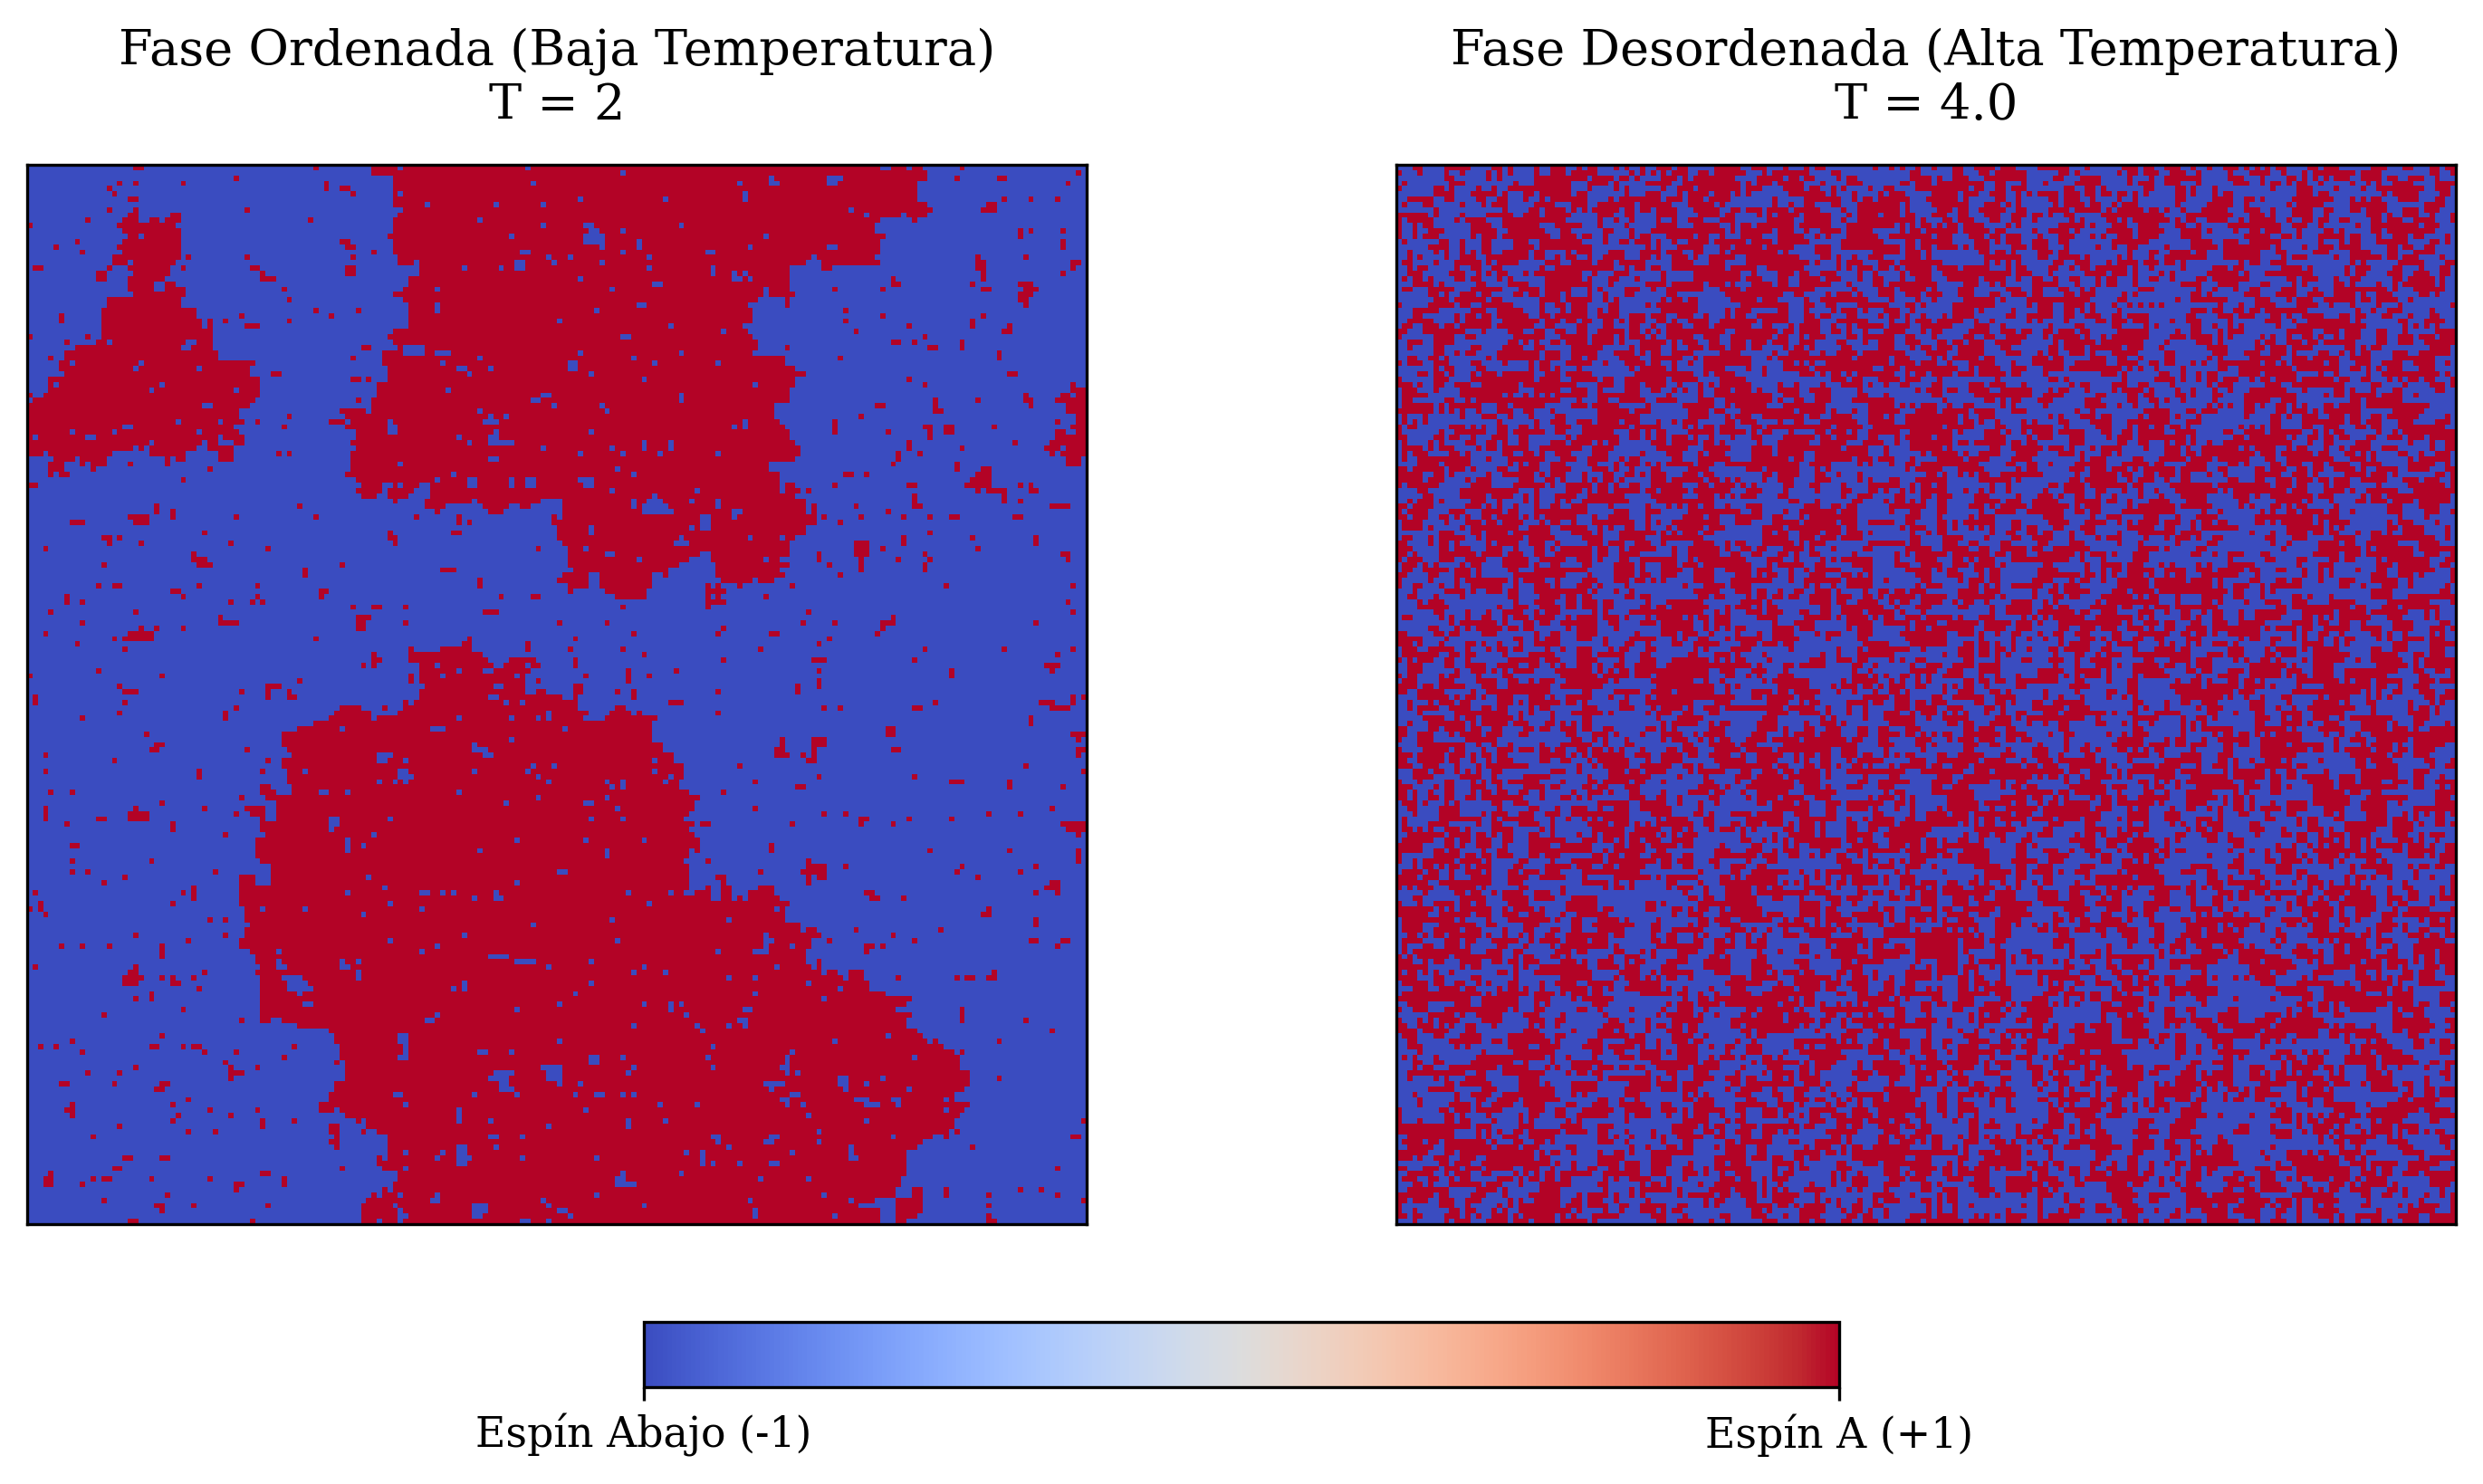
\includegraphics[width=0.8\linewidth]{Figures/transicion_fase_ising_corregida.png}
  \caption{Simulación del modelo de Ising para mostrar cómo para temperaturas menores a la temperatura crítica, \(T_c \simeq 2.269\), el sistema se encuentra ordenado minimizando la energía, y cómo para temperaturas mayores a la temperatura crítica el sistema se encuentra no magnetizado maximizando la entropía.}
  \label{fig:ising}
\end{figure}

Sin embargo cuando la temperatura se encuentra justamente en el punto en el que no domina la minimización de energía ni la maximización de entropía, donde el sistema está \emph{a punto} de magnetizarse pero no lo está aún, y el comportamiento es completamente diferente al de cualquiera de las otras dos fases decimos que estamos en el punto crítico caracterizado por una plétora de propiedades diferentes, todas ellas gobernadas por una simple relación no lineal: las leyes de potencias.

\begin{figure}[htbp]
  \centering
  \begin{subfigure}[c]{0.55\textwidth}
    \caption{}
    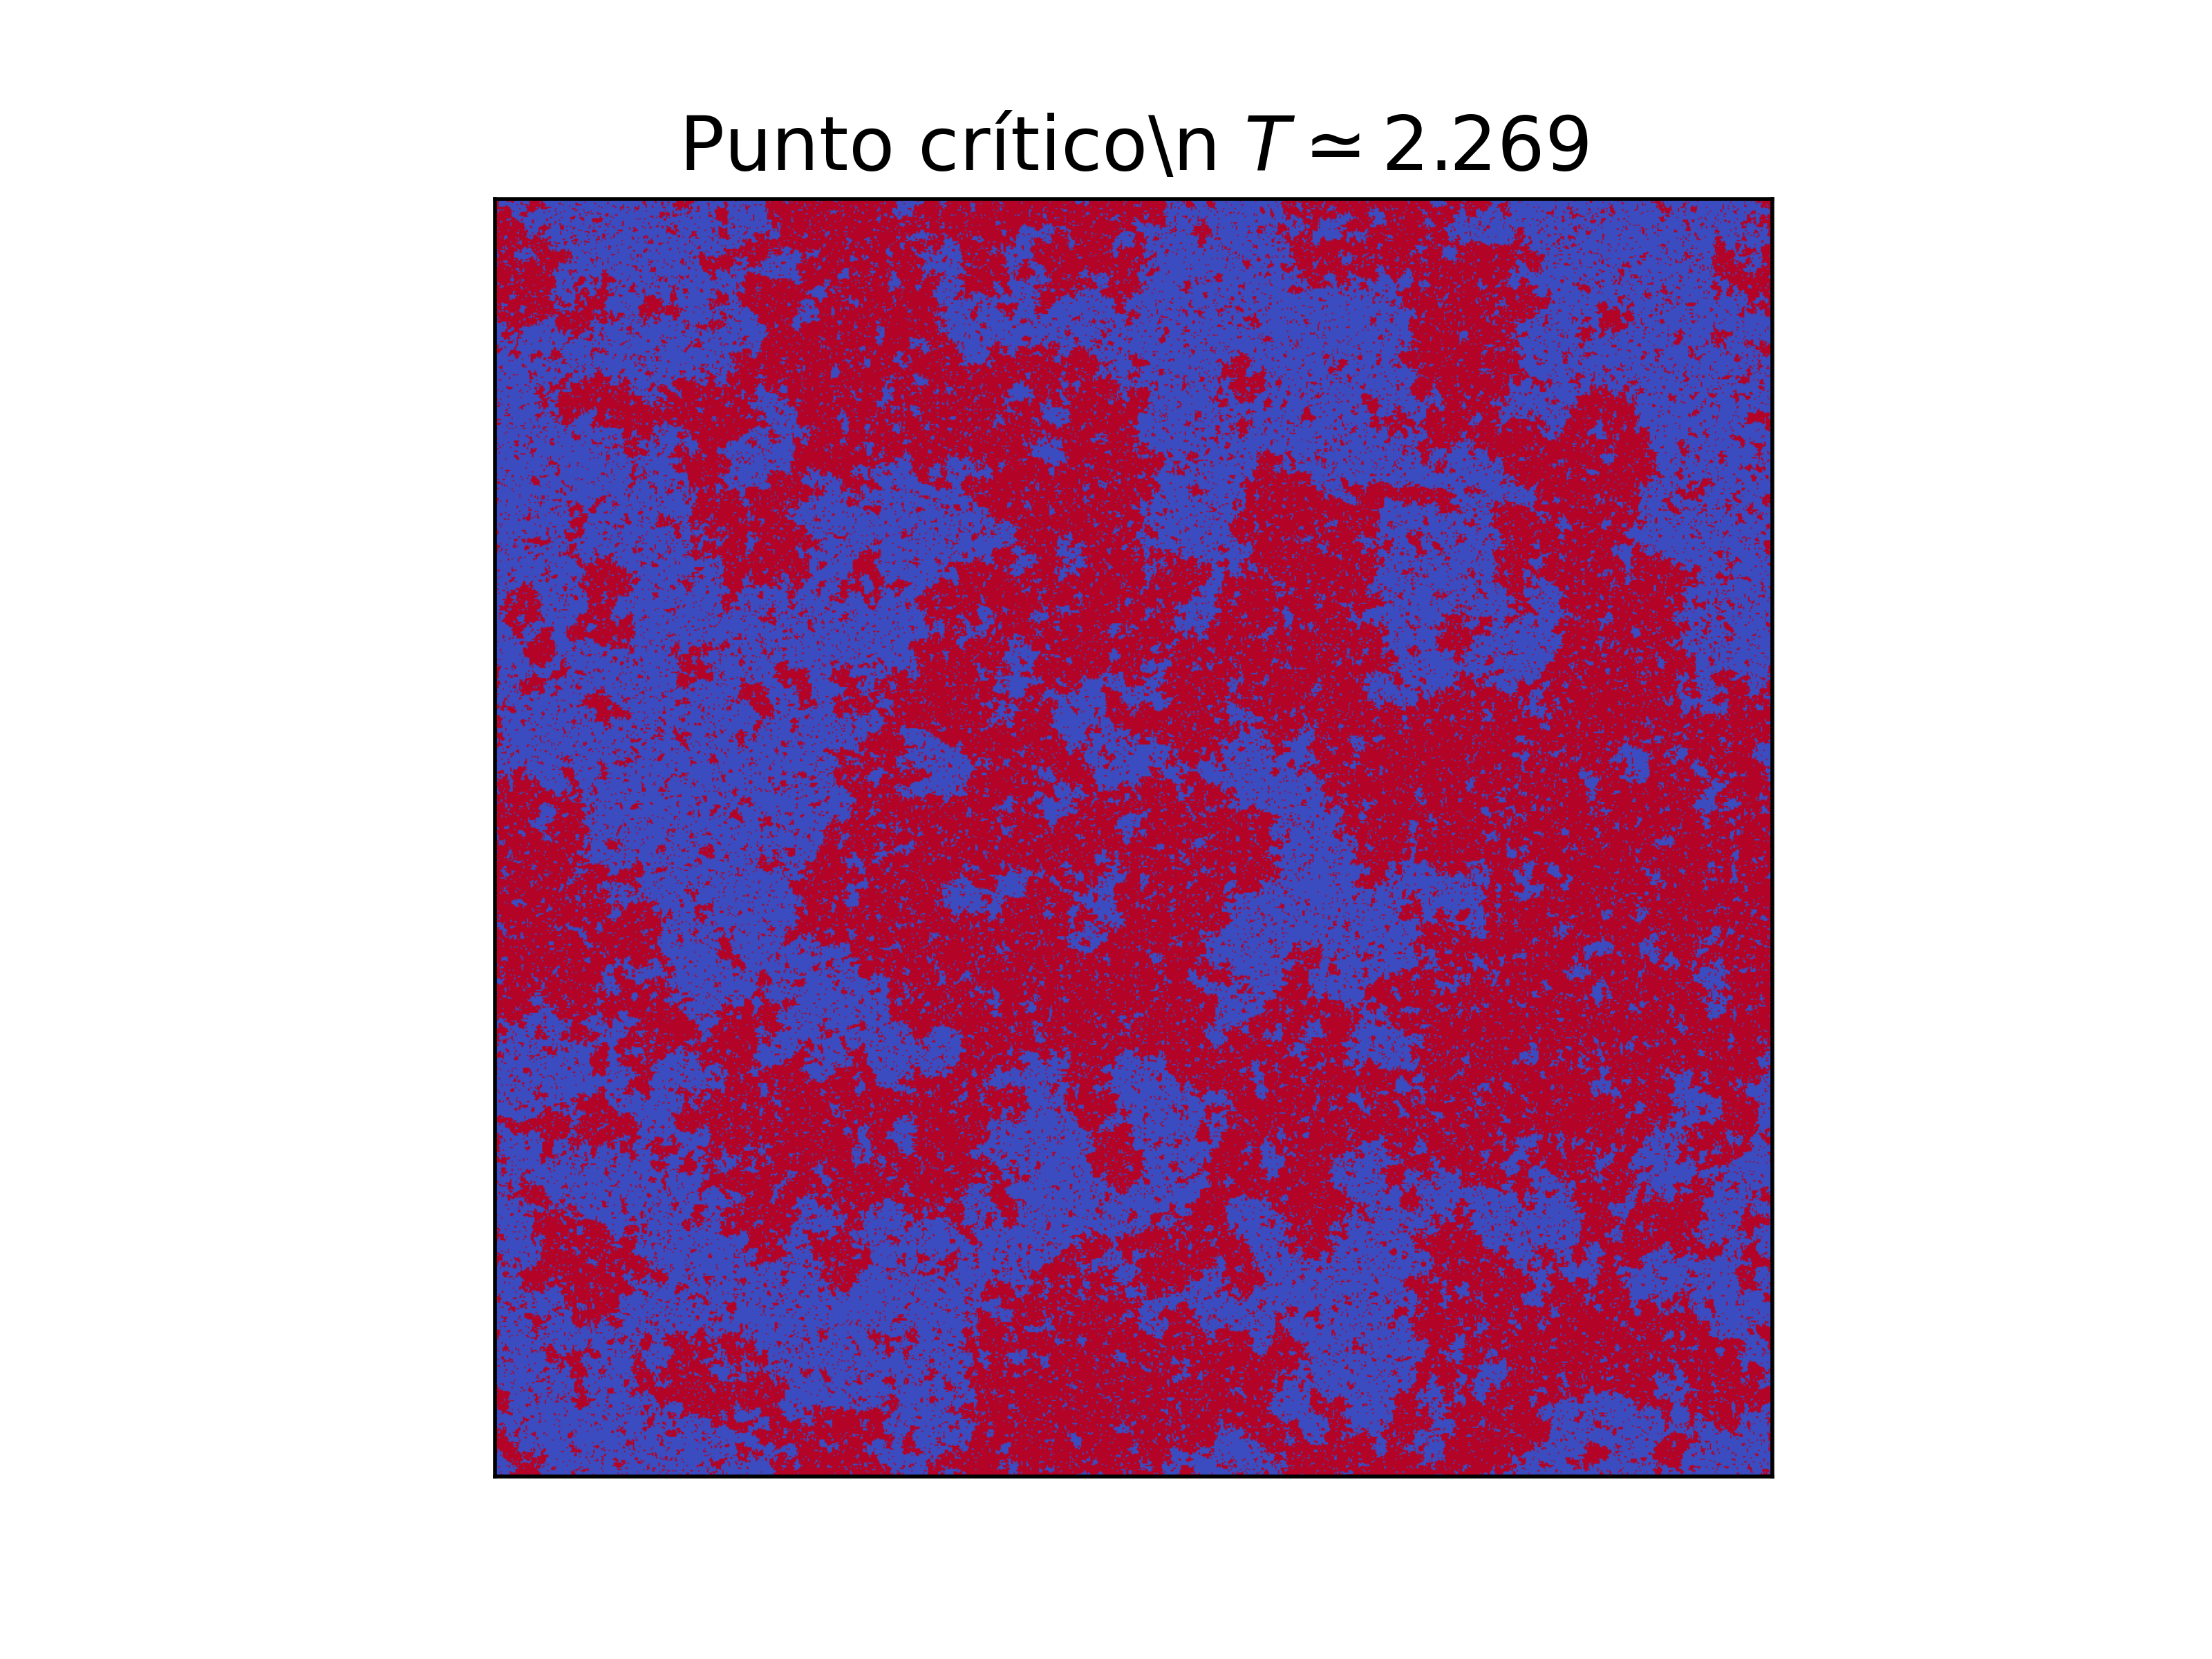
\includegraphics[width=\linewidth]{Figures/Ising_critico_sin_labels.png}
  \end{subfigure}
  \hfill
  \begin{subfigure}[c]{0.44\textwidth}
    \caption{}
    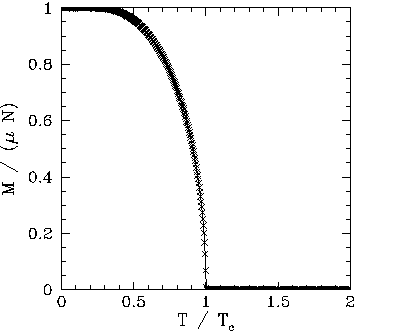
\includegraphics[width=\linewidth]{Figures/Magnetizacion.png}
  \end{subfigure}
  \caption{\textbf{Izquierda:} Modelo de Ising en el punto crítico. Se observa cómo en el punto crítico aparecen formaciones de todas las escalas, característica de un fractal. \textbf{Derecha:} Magnetización en función de la temperatura. Se observa cómo para \(T < T_c\) la magnetización es no nula creciendo desde 0, mientras que para \(T\ge T_c\) la magnetización es 0, situando al punto crítico se sitúa justo entre ambos regímenes.}
\end{figure}

El punto crítico se define por ser el punto en el que el parámetro del control, como la temperatura, es tal que el parámetro de orden, como la magnetización, es justo 0 al borde de la fase ordenada. En este punto las propiedades del material como la magnetización, el calor específico, la susceptibilidad magnética o la longitud de correlación siguen una ley de potencias frente a la temperatura

\begin{align}
    M(T) &\propto (T_c-T)^\beta\\
    C(T) &\propto |T_c-T|^\alpha\\
    \chi(T) &\propto |T_c-T|^{-\gamma}\\
    \xi(T) &\propto |T_c - T|^{-\nu}
\end{align}

Los exponentes que caracterizan el comportamiento de cada magnitud en torno al punto crítico se denominan exponentes críticos y lo interesante es que no dependen de las propiedades microscópicas del fenómeno, sino de la simetría que posea el parámetro de orden o la dimensión del sistema (1D, 2D, \(\dots\)), por lo que varios fenómenos en principio desconectados, como el modelo de Ising bidimensional y el cambio de fase entre líquido y gas por encima del punto crítico, tienen exactamente el mismo comportamiento cerca del punto crítico, por tanto algo sumamente útil a la hora de estudiar un sistema crítico será conocer sus exponentes, ya que estos determinan de forma unívoca la clase de universalidad a la que pertenecen.

\subsection{Criticidad auto organizada y cerebro crítico}
La región crítica en la mayoría de los sistemas se trata de una región de medida nula, generalmente un punto en la variedad definida por los parámetros de control, por lo que cualquier perturbación hace que un sistema que se encuentre en el punto crítico salga de este perdiendo las propiedades citadas, sin embargo a finales del siglo pasado varios investigadores \parencite{bak1987} sacaron a la luz cómo en ciertos sistemas como los terremotos, los incendios forestales o los granos que caen en una montañita de arena, \hl{poseen} propiedades como la magnitud de un terremoto, el tamaño de un incendio o el tamaño de las avalanchas de arena siguen una distribución de tipo ley de potencias similares a un punto crítico

\begin{equation}
  P(S) \propto S^{-\tau}
\end{equation}

A esta propiedad de alcanzar una dinámica gobernada por leyes de potencias sin necesidad de ajustar ningún parámetro de forma externa se le denominó criticidad auto organizada, (\emph{Self-Organized Criticality}), debido a que es la estructura del sistema la que impone que el parámetro de control, como el estrés acumulado en las placas tectónicas, la cantidad de combustible en el bosque o la pendiente de la pila de arena aumente hasta alcanzar un valor crítico por encima del cual se genera una \emph{avalancha} en setido general que disminuye el parámetro de control para que no supere ese valor crítico.

Dentro de dichos avances se encontró que para que dichos sistemas se auto organicen al punto crítico es necesario que la dinámica del parámetro de control venga modelada por un efecto de carga que aumente poco a poco el parámetro para acercarlo al punto crítico y un mecanismo de disipación que una vez alcanzado el punto crítico de active para disminuir el parámetro de control \parencite{buendia2020}. Estos dos mecanismos deben venir modulados por unas constantes de carga, \(h\), y disipación, \(\epsilon\), que cumplan \(h/\epsilon \rightarrow 0\) para que en la fase absorbente el parámetro de orden, sea 0, y \(h, \; \epsilon \rightarrow 0^+\) para separar las escalas temporales de la evolución del sistema y del control de este.
\begin{figure}[htbp]
  \centering
  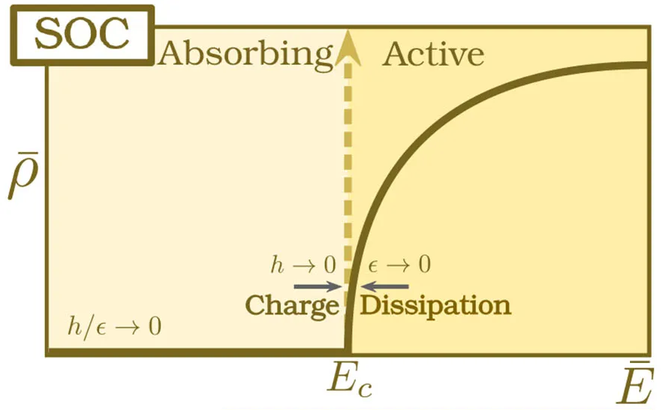
\includegraphics[width=.8\linewidth]{Figures/SOC serena.png}
  \caption{Esquema de la dinámica de un sistema SOC paradigmático donde las regiones activa y absorbente están separadas por un punto crítico en torno al que el sistema se localiza de forma automática mediante los mecanismos de carga y disipación extraído de  \parencite{buendia2020}.}
\end{figure}

Este tipo de criticidad se diferencia de la observada en modelos estáticos como el de Ising, donde el tiempo no representa un parámetro importante del sistema, pues el estado en el que se encuentra la red a una temperatura se considera estacionario, pues en los sistemas que exhiben criticidad auto organizada necesitan de la evolución constante del mismo para poder \emph{adaptarse} y modificar su comportamiento constantemente para estructurarse en torno a punto crítico. \hl{En este contexto aparece la criticidad dinámica}, pues ese choque entre fuerzas de excitación e inhibición perfectamente balanceadas es la que produce un estado sumamente suscetible ante pequeñas perturbaciones, situado entre la región absorbente, donde cada perturbación introducida en el sistema es anulada, y la región activa, que alimenta las perturbaciones hasta desestabilizar el sistema, en \hl{lo que se denomina el \emph{borde del caos} o \emph{borde de la criticidad}.
}

Tras estos descubrimientos gran cantidad de científicos intentaron aplicar la teoría de criticidad auto organizada para explicar diferentes fenómenos encontrados en la dinámica de las avalanchas de respuestas neuronales en el cortex del cerebro. \hl{En el contexto de la neurofísica nos referimos como avalanchas a picos de actividad en diferentes puntos de una sola región del cerebro a la vez, cómo si de un arbol de navidad se tratase, donde cada una de las luces es un punto donde se mide la actividad, se observó cómo a parte de aparecer picos individuales o de unas pocas luces encendiéndose a la vez también aparecen eventos a escalas mucho mayores en las que gran parte de la región se activa de forma simulatánea, comprobándose cómo el tamaño y la duración de las avalanchas seguían una distribución de probabilidad de ley de potencias} \parencite{beggs2003}, generando una \emph{avalancha} a su vez de investigaciones en neurofísica sobre la dinámica del cerebro. Parte de este cambio de paradigma a la hora de enfrentarse al estudio de los sistemas dinámicos terminó salpicando el terreno de las redes neuronales y la inteligencia artificial donde desde hace tan solo una década han empezado a generarse avances exponenciales en el desarrollo de nuevas tecnologías, y dentro de uno de estos avances de vanguardia se encuentran nuevos indicios de que las redes neuronales que trabajan en un régimen cercano al punto crítico (en el sentido dinámico, ni en una fase absorbente ni caótica) maximizan su capacidad de analizar y procesar información \parencite{bertschinger2004}.

{\color{blue}Bajo esta nueva tendencia aparecen estudios teóricos sobre la dinámica de las sinapsis. Las sinápsis son las conexiones entre las terminaciones nerviosas de las neuronas que se encargan de transmitir el impulso electroquímico entre ellas, excitando o inhibiendo su actividad dependiendo de las propiedades de la neurona emisora y receptora y de la propia conexión, pudiendo una misma neurona desencadenar un pico de actividad en una neurona vecina, pero apagar la de otra neurona diferente, solo debido a las características de la propia conexión. El modelo anti hebbiano es uno de estos modelos de control sinápico propuesto para estudiar si puede aparecer una autoorganización hacia un punto crítico, y qué beneficios o ventajas podría tener a la hora de emplearse en modelos de redes neuronales más complejas.}

\section{Fundamento teórico y metodología}
\subsection{Modelo lineal de dinámica neuronal y estabilidad}
\label{sec: Modelo lineal de dinámica neuronal y estabilidad}
Se va a emplear un modelo lineal de red neuronal en aras de simplificar el proceso de análisis y la interpretación de resultados, a pesar de la diferencia de la representación empleada con la realidad biológica. De este modo la actividad de la neurona \(i\) perteneciente a un sistema de \(N\) neuronas conectadas entre sí evoluciona según la ecuación
\begin{equation}
  \dot{x}_i = \sum_{j=1}^N w_{ij}x_j
\end{equation}
donde \(w_{ij}\) son los elementos de la matriz de conexiones \(W\). Esta ecuación puede ser escrita en forma matricial como 

\begin{equation}
  \dot{\mathbf{x}} = W\mathbf{x}
  \label{eq:evolución actividad}
\end{equation}

La matriz de conexiones que determina la evolución de \(\mathbf{x}\) puede, así mismo, variar con el tiempo según una dinámica que se dividirá en un término de estabilidad u homeostásis, \(\Delta_H\), y otro de aprendizaje, \(\Delta_L\).

\begin{equation}
  \dot{W} = \Delta_H + \Delta_L
  \label{eq:evolución conexiones}
\end{equation}

Parte del interés de estre trabajo radica en el estudio de la estabilidad de este sistema, dado que se busca un régimen en el que se comporte de forma similar a cómo se espera de un grupo de neuronas, sin que decaiga la actividad pero que tampoco explote. 

Se entiende como estabilidad de un sistema a la tendencia a la recuperación o modificación de la dinámica ante aparición de perturbaciones externas, ya sea debido al ruido o a las fluctuaciones propias de este. Para saber cómo responde la dinámica ante dicha alteración es útil estudiar la derivada que nos habla de cómo crece o disminuye dicha perturbación con el tiempo. Para ello es necesario encontrar los puntos estables del sistema que serán aquellos en los que no se producen cambios en el tiempo, que vendrán dados por

\begin{equation}
  \dot{\mathbf{x}} = 0\\
\end{equation}

Suponiendo que la conectividad es no nula, \(W\neq 0\), el único punto estable será \(\mathbf{x}^* = 0\). Al añadir una pequeña perturbación \(\mathbf{x} = \mathbf{x}^* + \bm{\delta}\), esta evolucionará según la dinámica

\begin{equation}
  \dot{\mathbf{x}} = \dot{\bm{\delta}} = W\bm{\delta}
\end{equation}

Por tanto al diagonalizar \(W\)\footnote{En los siguientes capítulos supondremos que \(W\) es una matriz aleatoria, por lo que la existencia de \(N\) autovalores complejos diferentes está asegurada con probabilidad 1 \parencite{mehta1991}} podemos escribir la evolución temporal de cada uno de los componentes de \(\bm{\delta}\) en la base de autovectores de \(W\). {\color{blue}Si tomamos \(\mathbf{v}_\lambda\) y \(\mathbf{u}^\dagger_\lambda\) como el los autovectores por la derecha e izquierda de \(W\) con autovalor \(\lambda\), la proyección de \(\bm{\delta}\) en la dirección de \(\mathbf{v}_\lambda\) sería \(\delta_\lambda = \mathbf{u}_\lambda^\dagger \bm{\delta}\)}, por lo que evolucionaría como

\begin{equation}
  \dot{\delta}_\lambda = \lambda \delta_\lambda \Rightarrow \delta_\lambda(t) = e^{\lambda t}\delta_\lambda (0)
\end{equation}

Por lo tanto para que el sistema sea estable, esto es para \(\bm{\delta}\) lo suficientemente pequeño \(\exists \epsilon \) tal que \( |\bm{\delta}(t)| < \epsilon, \; \forall t\), esto solo es posible si \(\re{(\lambda)} \le 0\), lo cual debe cumplirse para todos los autovalores. La parte imaginaria de \(\lambda\) lo único que hace en principio es añadir una fase de módulo 1 a la perturbación por lo que no afecta a la estabilidad del sistema, aunque sí a otras propiedades como se discutirá más adelante.

\begin{figure}[H]
  \centering
  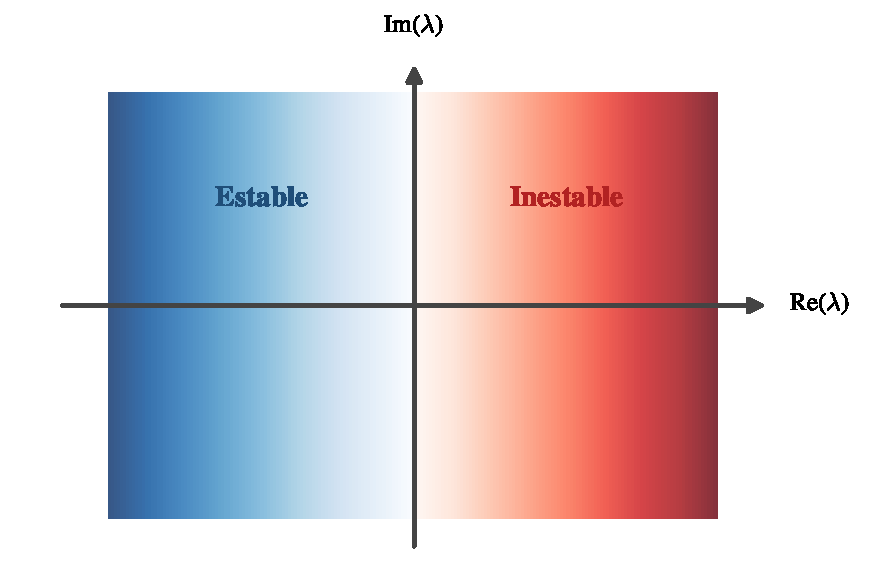
\includegraphics[width=.8\linewidth]{Figures/diagrama de estabilidad.pdf}
  \caption{Diagrama de estabilidad en el plano complejo del sistema \(\dot{x} = Wx\). La existencia de autovalores en la zona roja \(\re{(\lambda)}>0\) implica la inestabilidad del sistema, \hl{por lo que en este modelo el borde de la criticidad se encuentra justo en la zona blanca entre la región estable e inestable.}}
\end{figure}
\subsection{Modelo de Hopfield}
La matriz de conexiones \(W\) no se trata solamente de un término que determine la estabilidad del sistema, pues en esta reside fundamentalmente la dinámica \hl{de las sinápsis}, sirviendo sus \(N^2\) conexiones como parámetros que, al modificarlos y ajustarlos, pueden generar procesos similares al almacenamiento y generación de patrones basados en estímulos presentados a la red: recuerdos.

{\color{blue}El modelo de Hopfield, premio Nobel en física de 2024, se trata de uno de los modelos de red neuronal más simples que son capaces de almacenar y recuperar patrones; una forma híper simplificada de memorias o recuerdos \parencite{hopfield1982}. En el modelo de Hopfield se define una red \(\mathbf{x}\) de \(N\) nodos o neuronas cuyo estado individual viene descrito por una variable discreta, generalmente \(\pm 1\). Las neuronas se encuentran conectadas todas entre sí a través de una matriz \(W\), siendo la conexión entre la neurona \(x_i\) y la \(x_j\) el término \(W_{ij}\) de la matriz de conexiones. Cada una de estas conexiones puede tomar a su vez un valor de \(\pm 1\), siendo \(+1\) cuando la actividad de la neurona \(x_i\) genera actividad en la neurona \(x_j\) con el mismo signo, y siendo \(-1\) cuando genera el efecto contrario 

\begin{align}
  x_i &= +1 \stackrel{W_{ij}=+1}{\longrightarrow}x_j = +1\\
  x_i &= +1 \stackrel{W_{ij}=-1}{\longrightarrow}x_j = -1
\end{align}

La evolución de la red, por tanto, vendrá dada de la contribución neta de todas y cada una de las neuronas en ella

\begin{align}
  x_i &\rightarrow +1 \; si \sum_j W_{ij}x_j \ge 0\\
  x_i &\rightarrow -1 \; si \sum_j W_{ij}x_j < 0
  \label{eq:evolucion Hopfield}
\end{align}

Para almacenar una serie de \(P\) patrones \(\bm{\xi}^p\) de -1s y +1s para recuperarlo más tarde se lleva a cabo en la fase de aprendizaje la modificación de la matriz de conexiones de una forma concreta 

\begin{equation}
  W_{ij} = \frac{1}{P}\sum_{p=1}^P \xi_i^p\xi_j^p, \quad W_{ii} = 0
  \label{eq:regla aprendizaje hopfield}
\end{equation}
haciendo así que la información de los patrones almacenados quede guardada dentro de la propia estructura de la matriz de conexiones, que queda invariante durante el resto del proceso. Una vez aprendidos los patrones, si se inicializa a la red en un estado \emph{similar} al de alguno de ellos, esta es capaz, mediante el proceso de actualización de cada neurona, de converger al patrón deseado. Esto es posible debido a que cada uno de los patrones \(\bm{xi}^p\) es ahora un mínimo local de la energía de la red, definida como 

\begin{equation}
  E = -\frac{1}{2}\sum_{i,j}W_{ij}x_ix_j
  \label{eq:energia hopfield}
\end{equation}

donde se puede demostrar que la evolucón de \(\mathbf{x}\) según la regla \ref{eq:evolucion Hopfield} minimiza la energía de la red en cada paso. Sin embargo para asegurar la convergencia de la red son necesarias dos condiciones que deben cumplirse, una es que el número de patrones almacenados no sea demasiado alto, existe un límite a partir del cual los mínimos se empiezan a solapar y el sistema puede converger a patrones espúreos que no se hayan introducido específicamente, que para la regla de aprendizaje de la ecuación \eqref{eq:regla aprendizaje hopfield} es \(P \simeq 0.14 N\), y la otra es que los patrones no sean demasiado parecidos entre ellos para que los mínimos de la energía no sean demasiado cercanos y el sistema pueda diferenciar entre uno y otro.
}

\begin{figure}[htbp]
  \centering
  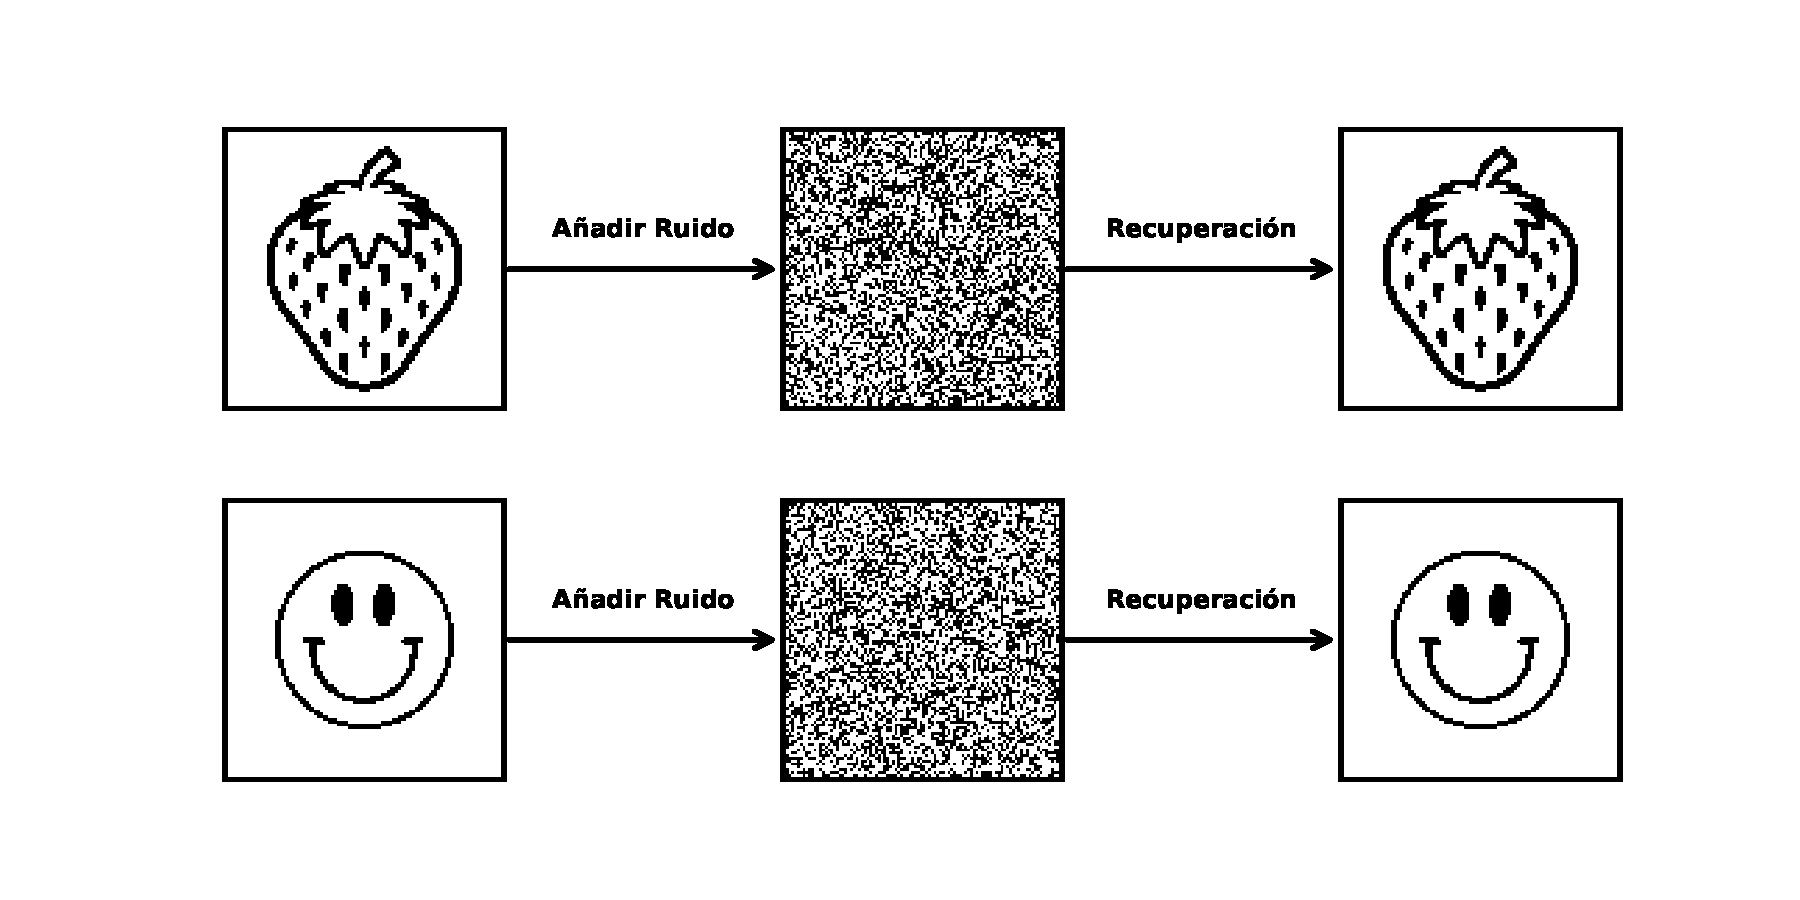
\includegraphics[width=\linewidth]{Figures/Hopfield.pdf}
  \caption{Una red neuronal de Hopfield es capaz de almacenar varias memorias y recuperarlas tras introducir un estímulo parecido. Añadimos dos patrones de memoria a la matriz de conexiones, una fresa y una carita feliz, y comenzamos con un vector de neuronas con cada uno de los dos patrones para luego añadirle ruido al patrón para que el sistema contenga la información del patrón original solo parcialmente. Presentándole este vector de 1s y -1s a la matriz de conexiones somos capaces, de una sola pasada, de recuperar totalmente el patrón original en ambos casos mediante la misma matriz de conexiones.}
\end{figure}

\subsection{Aprendizaje hebbiano}
La elección de \(W_{ij} = \xi_i \xi_j\) se le denomina regla de Hebb o aprendizaje hebbiano, ya que sigue la pauta propuesta por Donald Hebb \parencite{hebb1974}: \emph{Las neuronas que se activan juntas se conectan entre sí}\footnote{\emph{Neurons that fire together, wire together}.}. Esta regla establece que si dos neuronas tienen un pico de actividad a la vez la conexión entre ellas se fortalece, basada en propiedades conocidas de las conexiones sinápticas reales del cerebro, lo que en términos de la matriz de conexiones \(W\) se puede escribir como

\begin{equation}
  \dot{W} \propto \mathbf{xx}^T
\end{equation}

El principio de Hebb constituye una de las reglas básicas empleadas en redes neuronales artificiales para alterar las conexiones neuronales, pudiendo así obtener una estructura que posea propiedades del estímulo aplicado. Este tipo de dinámica constituye una forma muy básica de aprendizaje no supervisado sin necesidad de entrenamiento no lineal costoso, sin embargo debido a su simpleza la regla posee una limitación importante, y es que la dinámica emergente que genera en las neuronas hace que el sistema diverja exponencialmente.

Si suponemos nuestro sistema simplificado con \(W\) simétrica

\begin{align}
  \dot{\mathbf{x}} &= W\mathbf{x}\\
  \dot{W} &= \eta \mathbf{xx}^T
\end{align}

podemos estudiar cómo evoluciona \(q = |\mathbf{x}|^2\)

\begin{align}
  \dot{q} = 2x^T\dot{\mathbf{x}} = 2x^TW\mathbf{x}
\end{align}

derivamos una vez más aplicando la dinámica de \(\mathbf{x}\) y de \(W\)

\begin{align}
  \ddot{q} &= 2(\dot{\mathbf{x}}W\mathbf{x} + \mathbf{x}^T\dot{W}x + \mathbf{x}^TW\dot{x})\\
   &= 4(\mathbf{x}^TW^T)(W\mathbf{x}) + 2\mathbf{x}^T(\eta \mathbf{xx}^T)\mathbf{x}\\
   &= 4|W\mathbf{x}|^2+2\eta q^2
\end{align}

Por la desigualdad de Cauchy-Schwarz, sabemos que el término de la primera derivada elevado al cuadrado cumple que \(\dot{q}^2 = 4(x^TW\mathbf{x})^2 \le 4|\mathbf{x}|^2|W\mathbf{x}|^2\). Esto nos permite acotar \(|W\mathbf{x}|^2\) por abajo

\begin{equation}
  4|W\mathbf{x}|^2 \ge \frac{\dot{q}^2}{q}
\end{equation}

Sustituyendo esto en nuestra ecuación de \(\ddot{q}\), obtenemos la siguiente desigualdad diferencial

\begin{equation}
  \ddot{q} \ge \frac{\dot{q}^2}{q} + 2\eta q^2
\end{equation}

Si la resolvemos obtenemos la siguiente desigualdad para \(q(t)\)

\begin{equation}
  q(t) \ge e^{\eta t^2 + C_0 t}
\end{equation}

Siendo \(C_0 = \frac{\dot{q}(0)}{q(0)}\), por lo que la norma de los estados está acotada inferiormente por una función exponencial con exponente cuadrático, por lo que diverge a tiempo infinito adoptando valores extremadamente largos a corto tiempo. Este comportamiento hace que para mantener el aprendizaje durante largo tiempo sea necesario aplicar algún tipo de acotamiento para que el aprendizaje sea funcional, generando dinámicas como la regla de Oja \parencite{oja1982} o algoritmos hebbianos generalizados \parencite{sanger1989}. En nuestro caso el enfoque va a ser el opuesto, más que intentar añadir algún mecanismo que haga que el término hebbiano no haga explotar la dinámica emplearemos el propio término para estabilizar el sistema, basándonos en el trabajo de \textcite{magnasco2009} estudiaremos una dinámica anti hebbiana.

\subsection{Aprendizaje anti hebbiano}
Como se ha comprobado en la sección \ref{sec: Modelo lineal de dinámica neuronal y estabilidad} la búsqueda de estabilidad en el sistema \eqref{eq:evolución actividad} implica el control sobre la parte real de los autovalores de \(W\), para ello se tiene en cuenta que estos están \emph{asociados} a la parte simétrica de la matriz al igual que los imaginarios lo están a la antisimétrica \footnote{Con \emph{asociado} nos referimos a que las matrices simétricas (o hermíticas en general) sólo poseen autovalores reales mientras que las antisimétricas (antihermitianas) sólo imaginarios, además de que la parte real de los autovalores de una matriz está acotada por los autovalores de su parte simétrica e igual con la imaginaria \parencite{bendixson1902}.}.

Teniendo esto en cuenta se selecciona una dinámica que evite el crecimiento indefinido de la parte real de los autovalores limitando la parte simétrica de \(W\), \hl{por lo que empleando la dinámica de la regla de Hebb, pero empleando el signo opuesto} \parencite{magnasco2009} se consigue que el crecimiento de \(\mathbf{x}\) frene la evolución de \(W\) creando un ciclo de retroalimentación negativa. El término regulador de las conexiones de la ecuación \eqref{eq:evolución conexiones} sería

\begin{equation}
  (\Delta_H)_{ij} = \alpha(\delta_{ij} - x_i x_j)
\end{equation}
que en forma matricial se expresa como 

\begin{equation}
  \Delta_H = \alpha\left(\mathbb{1}_N - \mathbf{xx}^T\right)
  \label{eq:antihebbian rule}
\end{equation}
donde \(\alpha \ll 1\) es el parámetro de aprendizaje \footnote{Se añade la identidad en la ecuación \eqref{eq:antihebbian rule} para que una vez que \(|\mathbf{x}| \ll 1\) debido a la retroalimentación negativa \(W\) no siga disminuyendo hasta apagar el sistema y que se restaure la actividad poco a poco.}. Esta dinámica ha sido bautizada como anti hebbiana ya que al contrario que en la hebbiana podemos interpretar la dinámica como "\emph{Las neuronas que se activan juntas se desconectan entre sí}"

Al inicializar \(W\) con entradas aleatorias parte de los autovalores tendrán parte real positiva, por lo que en \(t \simeq 0\) la evolución de \(\mathbf{x}\) vendrá dictaminada por aquellos modos con \(\re(\lambda) > 0\). El módulo de dichos modos aumenta de forma drástica, por lo que el término \(-\mathbf{xx}^T\) de la matriz \(\dot{W}\) se hace muy negativa, lo que hace negativa a \(W\), haciendo que \(\mathbf{x}\) disminuya a su vez hasta valores cercanos a 0, en este momento el término \(\mathbb{1}\) se hace relevante y genera un crecimiento de \(W\) linealmente, que a su vez hace crecer \(\mathbf{x}\) {\color{blue}resultando en que la parte real de los autovalores de \(W\) quede oscilando cerca de 0} \parencite{magnasco2009} como se observa en la figura \ref{fig:dinamica anti hebbiana}.

\begin{figure}[htbp]
  \begin{subfigure}[t]{0.38\linewidth}
    \centering
    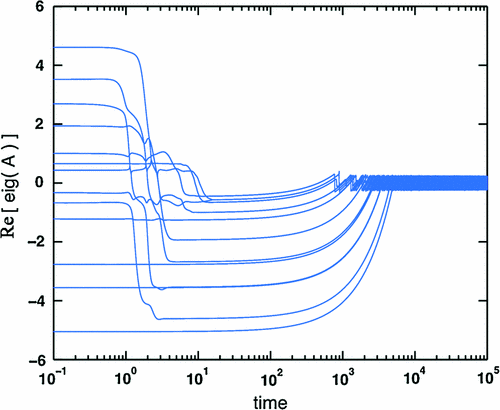
\includegraphics[width=\linewidth]{Figures/Magnasco real eigenvalues.png}
    \phantomcaption
    \label{fig:Evolucion parte real Magnasco}
  \end{subfigure}
  \hfill
  \begin{subfigure}[t]{0.6\linewidth}
    \centering
    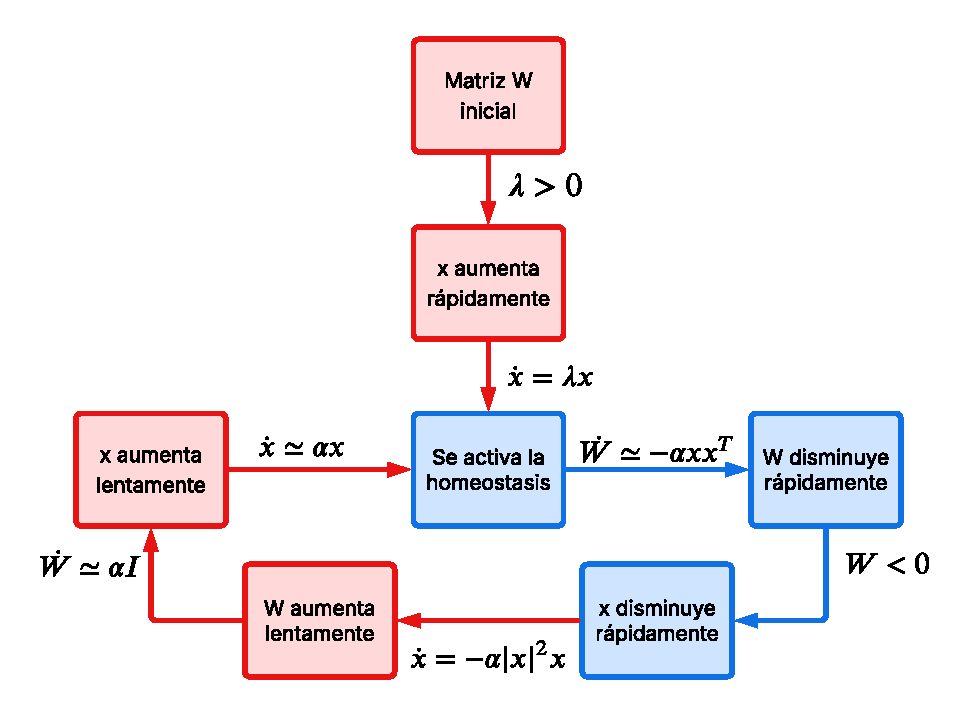
\includegraphics[width=\linewidth]{Figures/Flowchart.pdf}
    \phantomcaption
    \label{fig:diagrama de flujo}
  \end{subfigure}
  \caption{\subref{fig:Evolucion parte real Magnasco} Relajación de la parte real de los autovalores de la matriz \(W\) (llamada \(A\) en el eje de la figura) al hacer evolucionar el sistema con la dinámica anti hebbiana. Figura extraída de \parencite{magnasco2009}. \subref{fig:diagrama de flujo} Diagrama de flujo de la retroalimentación negativa entre \(W\) y \(\mathbf{x}\) generada por el aprendizaje anti hebbiano.}
  \label{fig:dinamica anti hebbiana}
\end{figure}

\subsection{Aprendizaje anti simétrico y STDP}
\label{sec:Aprendizaje anti simétrico y STDP}
La característica principal de que la dinámica que se encarga de estabilizar el sistema sea puramente simétrica implica que la parte antisimétrica de la matriz \(W\), \(A = \frac{W-W^T}{2}\), queda inalterada durante todo el proceso, \(\dot{A} = 0\), por lo que es interesante desarrollar algún tipo de dinámica que sea antisimétrica que nos permita almacenar información en la parte antisimétrica de \(W\). Para ello recurrimos a la ecuación \eqref{eq:evolución conexiones} donde el término \(\Delta_L\) se encarga de codificar la información entrante mediante cualquier tipo de estímulo y almacenarla en la matriz de conexiones de forma \emph{permanente} \parencite{susman2019}.

Siguiendo la estela del modelo de Hopfield, sería ideal que el término asociado a la memoria fuese capaz de almacenar un patrón y recuperarlo si se le proporciona un estímulo lo suficientemente parecido. Para ello de forma equivalente a cómo en el modelo de Hopfield la matriz de conexiones es simétrica con entradas dadas por \(\xi_i\xi_j\) siendo \(\bm{\xi}\) el vector cuya información deseamos almacenar, para obtener una matriz antisimétrica el rango debe ser al menos 2 por lo que construiremos nuestra matriz de la forma

\begin{equation}
  A = \rho(\mathbf{rs}^T - \mathbf{sr}^T)
\end{equation}

Para la construcción de dicha matriz recurrimos a un tipo de dinámica presente en ciertos tipos de aprendizaje que posee una direcccionalidad bien definida, la plasticidad dependiente del tiempo de disparo o STDP\footnote{Spike-time-dependent plasticity}. Esta regla determina que cuando la neurona presináptica \(x_i\) dispara antes que la post sináptica \(x_j\) la conexión en la dirección \(x_i \rightarrow x_j\) se refuerza mientras que la conexión en la dirección contraria \(x_j \rightarrow x_i\) se debilita, haciendo que \(W_{ij}\) y \(W_{ji}\) se modifiquen de forma opuesta, lo que podemos aproximar como una alteración antisimétrica de \(W\). Para ello se propone un método basado en \textcite{susman2019} en el que se toma 
\begin{align}
  \Delta_L &= \eta \left(\mathbf{xy}^T - \mathbf{yx}^T\right)\\
  \dot{\mathbf{y}} &= \frac{1}{\tau}(\mathbf{x}(t) - \mathbf{y})
\end{align}

El término \((\Delta_L)_{ij}\) representa la conexión en la dirección \(x_j \rightarrow x_i\) siendo \(\mathbf{y}\) la actividad de las neuronas suavizada mostrando un eco o rastro de la actividad de cada neurona en tiempos anteriores, por lo que si a tiempo \(t\) la neurona \(x_j\) ha disparado hace poco \(y_j\) será grande y por lo tanto si \(x_i\) está disparando \(x_i y_j\) será grande también, pero si ocurre al revés y es la neurona post sináptica \(x_i\) la que ha disparado antes \(y_i\) será grande y al estar disparando \(x_j\) el término \(x_jy_i\) será el que domine. 

\begin{equation}
  (\Delta_L)_{ij} = \eta \Big( \underbrace{x_i y_j}_{\substack{\text{Causal:} \\ j \text{ dispara antes que } i}} - \underbrace{x_j y_i}_{\substack{\text{Anti-causal:} \\ i \text{ dispara antes que } j}} \Big)
\end{equation}

Al añadirle a la dinámica de las neuronas un estímulo \(\mathbf{s}(t)\) \hl{suficientemente grande} generado por la combinación lineal de dos vectores \(\mathbf{r}\) y \(\mathbf{s}\) de la forma \(\mathbf{s}(t) = p_\mathbf{r}(t) \mathbf{r} + p_\mathbf{s}(t) \mathbf{s}\), siendo \(p_\mathbf{r}(t)\) y \(p_\mathbf{s}(t)\) escalares que dependen del tiempo. Una vez pasado un tiempo \(t\simeq \tau\) el vector \(\mathbf{y}\) se encontrará mayormente embabido en el plano \(\mathbf{rs}\) al igual que \(\mathbf{x}\), por lo que el término de aprendizaje se podrá expresar, con algunos matices, como 

\begin{equation}
  \Delta_L = \rho(\mathbf{rs}^T - \mathbf{sr}^T)
\end{equation}

Como se verá más adelante dicha aproximación resultará útil para obtener resultados significativos ya que el planteamiento expuesto por \parencite{susman2019} presenta varios problemas que se comentarán en las siguientes secciones.

\section{Resultados y discusión}
\subsection{Teoría de matrices aleatorias y existencia de \(N\) autovalores diferentes}
Es útil suponer que la estructura inicial de \(W\) no es clave para su evolución, por lo que inicializaremos las conexiones \(w_{ij}\) mediante elementos extraidos de una distribución normal \(\mathcal{N}(0, \sigma)\) para simular una condición inicial con el sistema \emph{no entrenado}. Dicha matriz \(W(t=0)\) posee autovalores distribuidos en el plano complejo de forma uniforme en el círculo de radio \(\sigma\sqrt{N}\) para \(\lim_{N\rightarrow \infty}\) según la ley circular \parencite{tao2010}, lo que asegura que existan autovalores con parte real positiva que \emph{enciendan} el proceso de homeostásis.

\begin{figure}[H]
  \centering
  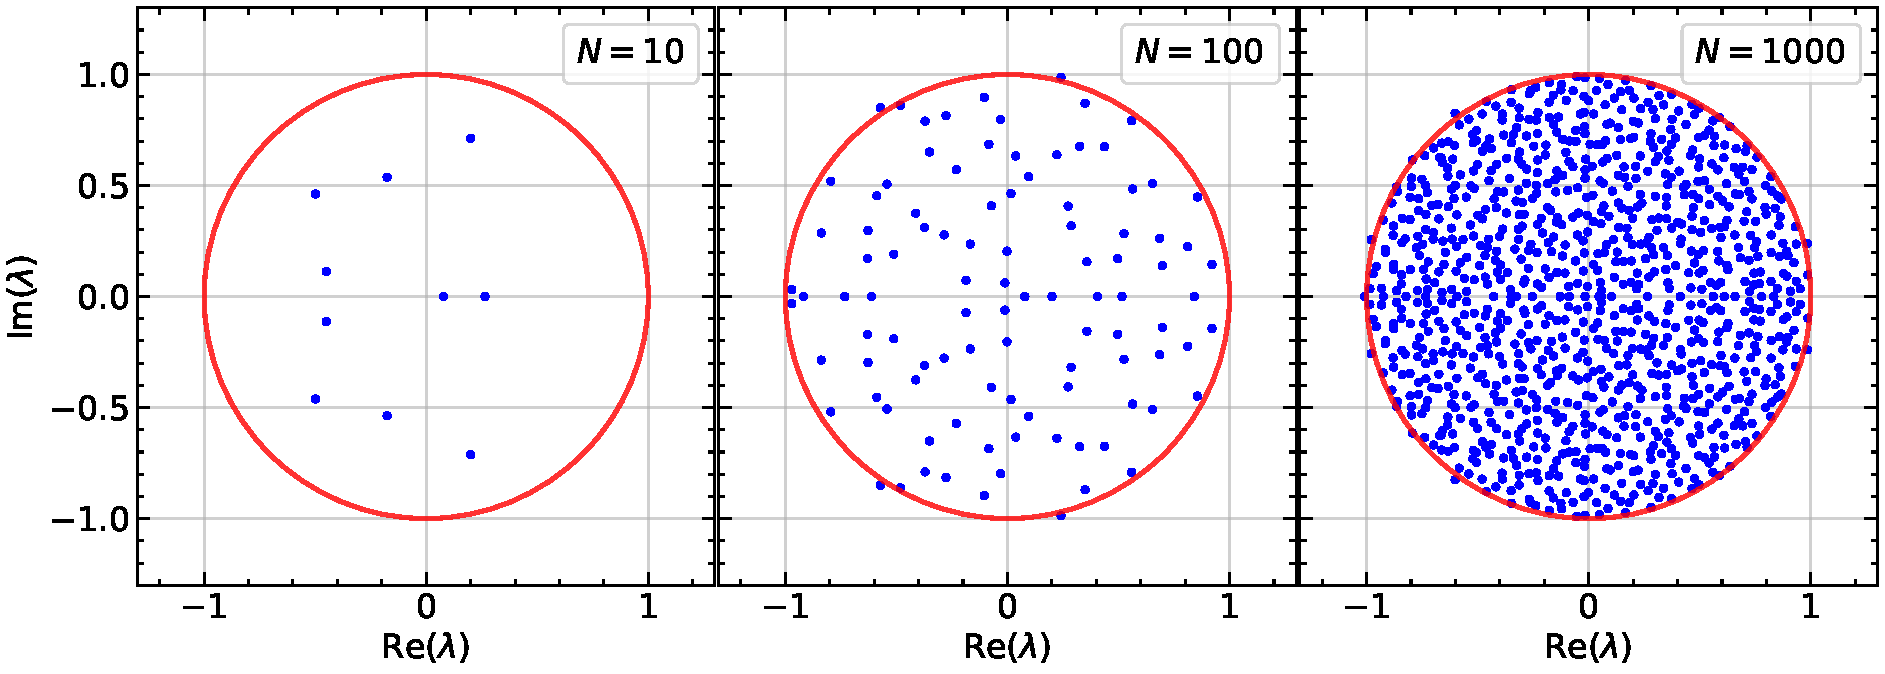
\includegraphics[width=\linewidth]{Figures/circular law.pdf}
  \caption{Espectro de una matriz con entradas \(W_{ij}\) que siguen una distribución \(\mathcal{N}\left(0, \frac{1}{\sqrt{N}}\right)\) para \(N = 10, \; 100, \; 1000\) donde se muestra como se cumple la ley circular a medida que aumenta \(N\), la dimensión de la matriz.}
\end{figure}

Al conjunto de matrices cuadradas reales con entradas independientes e idénticamente distribuidas según la distribución normal estándar se le denomina la colectividad de Ginibre, de la que se conocen una gran cantidad de propiedades \parencite{ginibre1965} \parencite{mehta1991}, lo cual es sumamente útil para explicar las propiedades de nuestro sistema, como la existencia con probabilidad 1 de \(N\) autovalores complejos diferentes, sin embargo el análisis empleado no depende de la elección en la inicialización de la matriz ya que como la dinámica de \(W\) añade un término perturbativo que depende de \(\mathbf{x}\), el cual inicialmente se ha obtenido de forma aleatoria, se puede demostrar que la matriz perturbada \(W + \delta W\) es diagonalizable con probabilidad 1, ya que el conjunto de matrices diagonalizables con autovalores diferentes es denso en el conjunto de todas las matrices \parencite{horn1985}.

Sin embargo aunque la existencia de \(N\) autovalores diferentes implique la existencia de \(N\) autovectores \(\mathbf{v}\) tal que

\begin{equation}
  W\mathbf{v} = \lambda \mathbf{v}
\end{equation}

Al escoger la matriz \(W\) de forma aleatoria la probabilidad de que sea normal, esto es \([W,W^T]=0\), es 0 \parencite{mehta1991}, por lo que los autovectores no serán ortogonales entre sí, solo linealmente independientes\footnote{Concretamente si \(W\) es normal los \(N\) autovectores formarán una base ortogonal del espacio de Hilbert \((\mathbb{C}^N, \mathbb{C}, \braket{\cdot}{\cdot})\)}, por lo que la descomposición ortogonal de \(\mathbf{x}\) en autovectores de \(W\) deberá tener en cuenta los autovectores por la izquierda de \(W\), \(\mathbf{u}\), que cumplen

\begin{equation}
  \mathbf{u}^\dagger W = \lambda \mathbf{u}^\dagger
\end{equation}
ya que para estos dos conjuntos de vectores es posible aplicar la condición de biortoginalidad

\begin{equation}
  \mathbf{u}_\lambda^\dagger \mathbf{v}_{\lambda'} = \delta_{\lambda \lambda'} \Rightarrow \mathbb{1} = \sum_{\lambda} \mathbf{v}_\lambda \mathbf{u}_\lambda^\dagger
\end{equation}
por tanto la descomposición de \(\mathbf{x}\) en autovectores de \(W\) sería

\begin{equation}
  \mathbf{x} = \sum_\lambda p_\lambda \mathbf{v}_\lambda, \quad p_\lambda = \mathbf{u}_\lambda^\dagger \mathbf{x}
\end{equation}

Esta descomposición nos será útil más adelante para estudiar cómo cada uno de los autovectores de \(W\) evoluciona de forma aproximadamente independiente.

\subsection{Dinámica de autovalores de la red y criticidad dinámica}
En primera instancia se ha llevado a cabo un estudio en profundidad del sistema, haciendo evolucionar \(\mathbf{x}\) mediante la ecuación \eqref{eq:evolución actividad} y \(W\) solo mediante el aprendizaje anti hebbiano \eqref{eq:antihebbian rule} buscando replicar los resultados de \textcite{magnasco2009} sobre la dinámica de la parte real de los autovalores \ref{fig:Evolucion parte real Magnasco} y la existencia de criticidad dinámica en la actividad de las neuronas.

Para obtener una intuición de cómo afecta la retroalimentación negativa a la actividad y las conexiones es útil estudiar el sistema unidimensional y entender los resultados que arroja: una neurona que se excita y se inhibe a sí misma

\begin{align}
  \dot{x} &= Wx\\
  \dot{W} &= \alpha(1 - x^2)
\end{align}
como ahora el sistema es unidimensional podemos calcular la primera integral, que será una constante del movimiento

\begin{align}
  \frac{dW}{dx} &= \frac{\dot{W}}{\dot{x}} = \frac{\alpha(1-x^2)}{Wx}\Rightarrow\\
  WdW &= \alpha\left( \frac{1}{x} - x \right)dx \Rightarrow\\
  H(x, W) &= \frac{1}{2}W^2 + \alpha\frac{1}{2}x^2-\alpha\ln|x| \label{eq:hamiltoniano}
\end{align}

Como podemos observar la ecuación \eqref{eq:hamiltoniano} representa el Hamiltoniano de un oscilador no lineal con una repulsión fuerte en torno a \(x=0\), por lo que las soluciones en \(x\) y \(W\) serán oscilatorias. Para el sistema multidimensional no es posible encontrar una constante del movimiento\footnote{Estrictamente sí conocemos una constante del movimiento, que es la parte antisimétrica de la matriz de conexiones, \(A = \frac{W-W^T}{2}\), ya que la regla anti hebbiana es simétrica, pero no nos habla de la dinámica de \(\mathbf{x}\) y \(W\).}, sin embargo el sistema seguirá el mismo patrón de oscilaciones como comprobaremos más adelante. Igualmente, aunque para el sistema unidimensional sí tenemos soluciones analíticas para \(x\) y \(W\) en función de las funciones \(\mathcal{P}\) de Weierstrass, para el sistema con dimensión \(N>1\) no es posible encontrar una solución exacta. El problema reside en que cuando aumentamos la dimensión aparecen las interacciones entre las neuronas y con los diferentes elementos de la matriz de conexiones, que al ser no lineales, no podemos despejar para encontrar constantes del movimiento, además tanto \(\mathbf{x}\) como \(W\) dejan de ser periódicas como en el caso unidimensional, figura \ref{fig:norma diferentes dimensiones}, y pasan a tener un comportamiento aparéntemente desordenado.
\begin{figure}[htbp]
  \centering
  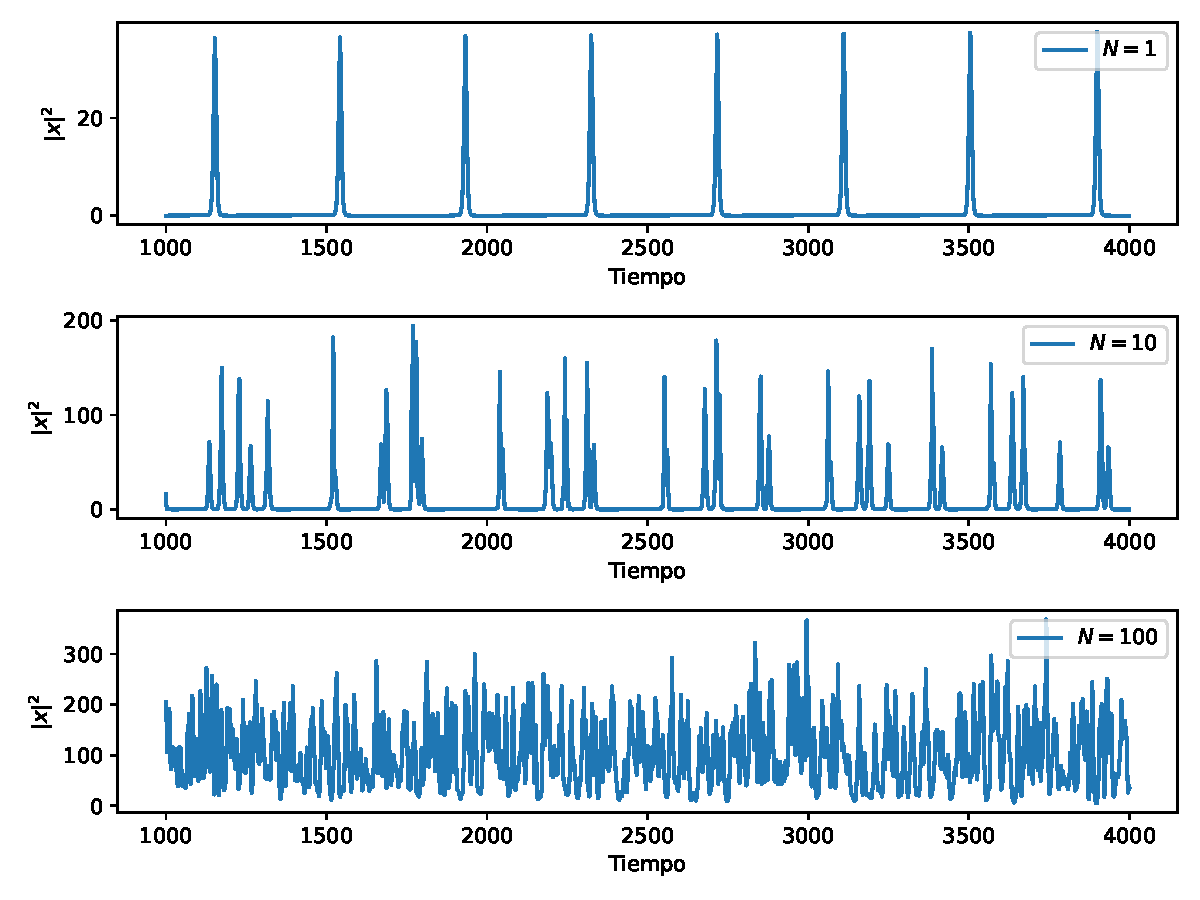
\includegraphics[width=\linewidth]{Figures/Norma X diferentes dimensiones.pdf}
  \caption{Evolución de \(|\mathbf{x}|^2\) para diferentes dimensiones del sistema una vez que se ha pasado el transitorio. Para \(N=1\) el sistema tanto en \(x\) como en \(W\) es periódico y con solución analítica en función de las funciones \(\mathcal{P}\) de Weierstrass, pero una vez que \(N>1\) la periodicidad se pierde y \(|\mathbf{x}|^2\) parece componerse de muchos picos diferentes en vez de un tren de picos iguales hasta llegar a fundirse entre ellos para \(N \gg 1\).}
  \label{fig:norma diferentes dimensiones}
\end{figure}

En cuanto a la dinámica de los autovalores que es mencionada en \textcite{magnasco2009}, se ha conseguido replicar la figura \ref{fig:Evolucion parte real Magnasco} del paper mencionado con datos propios, observando en la figura \ref{fig:evolución autovalores} cómo antes de producirse las oscilaciones en la parte real de los autovalores, aquellos con parte real mayor que 0 caen rápidamente hasta tener parte real menor que 0, y los autovalores reales con parte real menor que 0 aumentan linealmente (que en diagrama logarítmico se aprecia como exponencial) con pendiente \(\alpha\). Además, a diferencia de en el paper, observamos como la parte imaginaria se mantiene mínimamente perturbada como esperábamos debido a que la parte antisimétrica de \(W\) se mantiene constante, sin embargo no es posible estudiar la parte imaginaria de los autovalores únicamente con la parte antisimétrica de la matriz ya que no es cierto que los autovalores de \(A = \frac{W-W^T}{2}\) sean la parte imaginaria de los autovalores de \(W\), aunque sirvan para acotarlos \parencite{bendixson1902}. Una vez atravesado el transitorio observamos cómo los autovalores oscilan en torno al 0, de forma esperada debido a que la estabilidad del sistema requiere que no haya autovalores que se mantengan con parte real mayor que 0 de forma indefinida.

\begin{figure}[H]
  \centering
  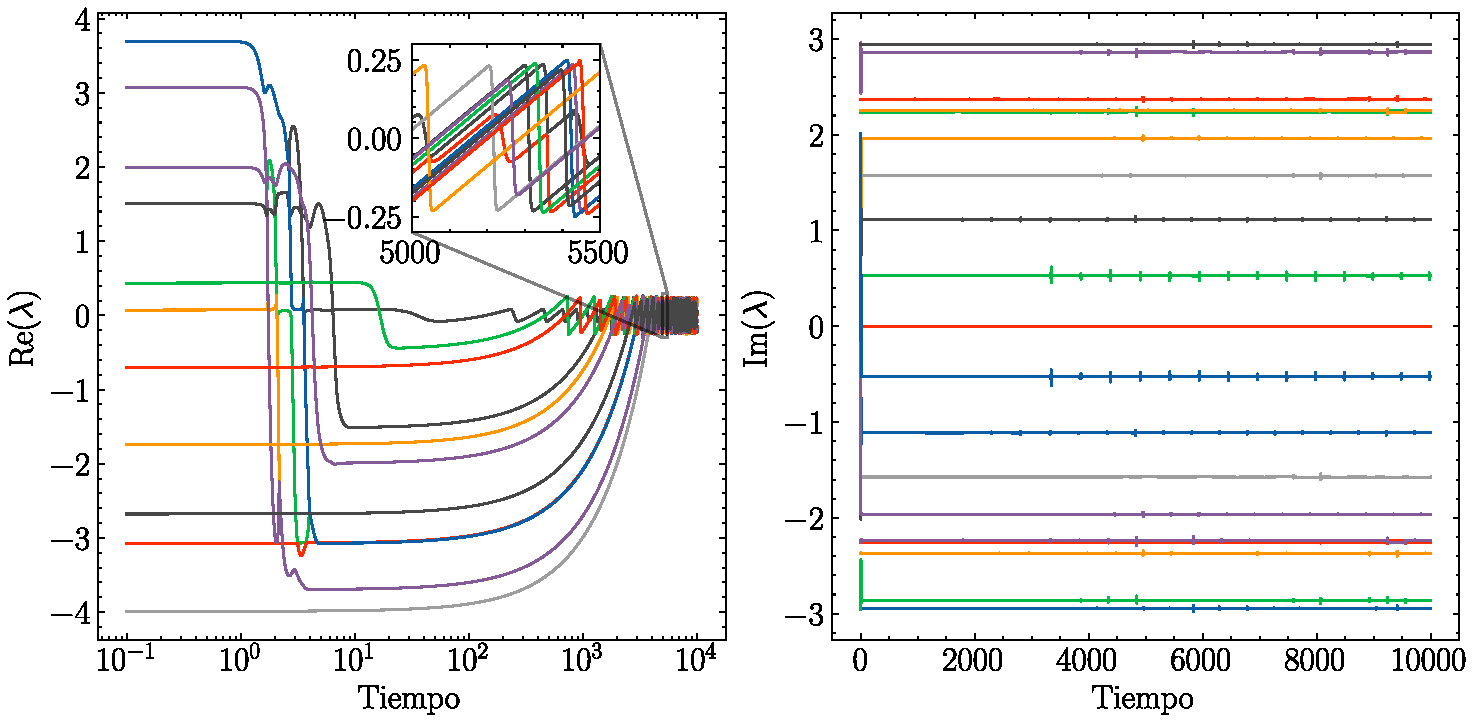
\includegraphics[width=\linewidth]{Figures/Evolucion coloreada.pdf}
   \caption{Evolución temporal de la parte real (\textbf{Izda.}) e imaginaria (\textbf{Dcha.}) de los autovalores de la matriz de conexiones, \(W\), con \hl{condición inicial} \(W_{ij}\sim \mathcal{N}(0, 1)\), para \(N=20\), \(\alpha = 0.001\). La parte real de los autovalores positivos disminuye rápidamente en escala de tiempo \(t_{+} \simeq 1\), mientras que la parte negativa aumenta hasta 0 en escalas de \(t_{-} \simeq 10^3 = \frac{1}{\alpha}\), mientras que para tiempos mayores que \(t_{-}\) la parte real oscila en torno a 0. La parte imaginaria se mantiene constante en promedio excepto por ligeras perturbaciones que ocurren cuando la parte real del autovalor alcanza el máximo en las oscilaciones.}
   \label{fig:evolución autovalores}
\end{figure}

Sin embargo a pesar de que el sistema aparenta ser caótico y desordenado a aumentar la dimensión debido a las interacciones, es posible \emph{desacoplar} el vector \(\mathbf{x}\) en las componentes de los autovectores de \(W\) y escribir el sistema \emph{desacoplado} en función de las variables \(p_\lambda = \mathbf{u}_\lambda^\dagger \mathbf{x}\), \(\tilde{p}_\lambda = \mathbf{v}_\lambda^\dagger \mathbf{x}\) y \(q_\lambda = \mathbf{u}_\lambda^\dagger \dot{x}\) como 

\begin{align}
  q_\lambda &= \lambda p_\lambda\\
  \dot{\lambda}_\lambda &= \alpha(1-p_\lambda\tilde{p}_\lambda^*) \label{eq:evolucion lambda}
\end{align}

Donde se ha empleado que \(\dot{\lambda} = \mathbf{u}_\lambda^\dagger \dot{W}\mathbf{v}_\lambda\) \parencite{greenbaum2020}. Hay que notar que la primera ecuación no relaciona \(p_\lambda\) con su derivada, \(\dot{p}_\lambda\), sino \(\mathbf{x}\) y \(\dot{\mathbf{x}}\) en la dirección del autovector \(\mathbf{v}_\lambda\), esto es importante porque la derivada de \(p_\lambda\) no es \(q_\lambda\), sino un término mucho más complicado que requiere calcular la derivada de los autovectores, aunque para \(\alpha \rightarrow 0\) y \(N\) no muy grande

\begin{equation}
  \frac{dp_\lambda}{dt} = \frac{d}{dt}(\mathbf{u}_\lambda^\dagger \mathbf{x}) = \dot{\mathbf{u}}_\lambda^\dagger \mathbf{x} + \mathbf{u}_\lambda^\dagger \dot{\mathbf{x}} = \sum_{\lambda'\neq \lambda}\frac{\mathbf{u}_\lambda^\dagger \dot{W}\mathbf{v}_{\lambda'}}{\lambda - \lambda'}\mathbf{u}_{\lambda'}^\dagger \mathbf{x} + \mathbf{u}_\lambda^\dagger \dot{\mathbf{x}} = -\sum_{\lambda'\neq \lambda}\alpha \frac{p_\lambda \tilde{p}_{\lambda'}^*}{\lambda - \lambda'}p_{\lambda'} + q_\lambda \stackrel{\alpha \rightarrow 0}{\simeq} q_\lambda
\end{equation}

Además \(\tilde{p}_\lambda \neq p_\lambda\) ya que \(\mathbf{u}_\lambda \neq \mathbf{v}_\lambda\) para matrices no normales, por eso la proyección del sistema en cada uno de las direcciones de los \hl{autovectores} no se comporta \hl{exactamente} con la dinámica unidimensional discutida antes, aún así para \(N \sim O(1)\), generalmente menor que 10 o 20, es lo suficientemente parecida como para poder suponer que la dinámica de \(\mathbf{x}\) viene dada por la suma de \(N\) dinámicas unidimensionales.

Siguiendo este análisis unidimensional, los picos en \(p_\lambda\) implican, mediante la ecuación \ref{eq:evolucion lambda}, \(\re(\dot{\lambda}) \ll 0\), esto es que las \emph{caídas} en la parte real de un autovalor se corresponden con picos en el modo asociado a ese autovalor y vice versa.

En la figura \ref{fig:picos} se observa este efecto, donde cada una de las \emph{caidas} en la parte real de los autovalores está asociada a un pico en la actividad de la proyección de \(\mathbf{x}\) sobre el autovector asociado a dicho autovalor y, de la misma forma, un pico en \(|\mathbf{x}|^2\).


\begin{figure}[htbp]
  \centering
  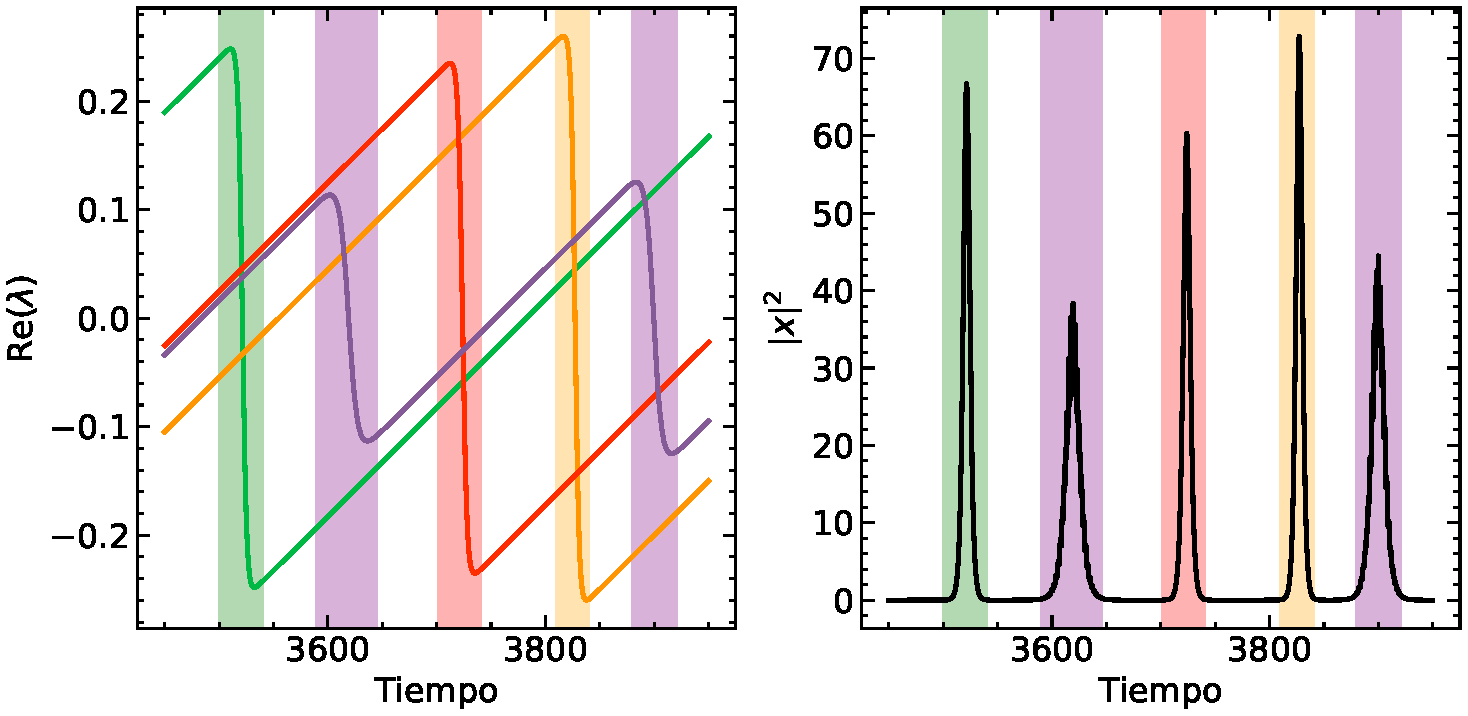
\includegraphics[width=\linewidth]{Figures/Picos.pdf}
  \caption{\textbf{Izquierda.} Evolución de la parte real de los autovalores de \(W\) con el tiempo. Se observa cómo oscilan en torno a \(\re(\lambda)=0\) con diferentes amplitudes. El autovalor morado se corresponde con un par complejo conjugado, mientras que el resto son autovalores puramente reales. \textbf{Centro.} Evolución de la proyección de \(\mathbf{x}\) sobre cada uno de los autovectores asociados a los autovalores de la primera imagen, se observan picos pronunciados que se corresponden temporalmente con \emph{caidas} en la parte real de los autovalores. \textbf{Derecha.} Evolución de \(|\mathbf{x}|^2\) donde se observan los mismos picos que en las proyecciones de \(\mathbf{x}\), pudiendo aproximar \(|\mathbf{x}|^2 \simeq \sum_\lambda |p_\lambda|^2\) ya que para \(N \sim 1\) los autovectores son \emph{casi} ortogonales y \(W\) es \emph{casi} normal. Simulación para \(N = 5\) y \(\alpha = 0.001\).}
  \label{fig:picos}
\end{figure}

Según \(N\) aumenta, la aproximación unidimensional se hace cada vez más menos adecuada y los términos cruzados de las proyecciones entre autovectores se hacen no despreciables en \(|\mathbf{x}|^2\), figura \ref{fig:picos acoplados}, además de que cuanto mayor es la dimensión mayor es la densidad de autovalores en la región del plano complejo donde se mueven estos, \hl{la \emph{cinta} estrecha y alargada }centrada en el eje imaginario, cuya aglomeración implica que los autovectores se hacen casi colineales entre sí \parencite{trefethen2005}. Este aumento en la población de los autovalores en la región crítica, en torno a \(\re(\lambda)=0\), hace que estos \emph{choquen} e interactúen entre sí desviándose del modelo de autovalores independientes aplicado para dimensiones bajas, de forma análoga a cómo al aumentar la densidad el modelo de gas ideal debe ser corregido mediante interacciones como en el de Van der Waals.

\begin{figure}[htbp]
  \centering
  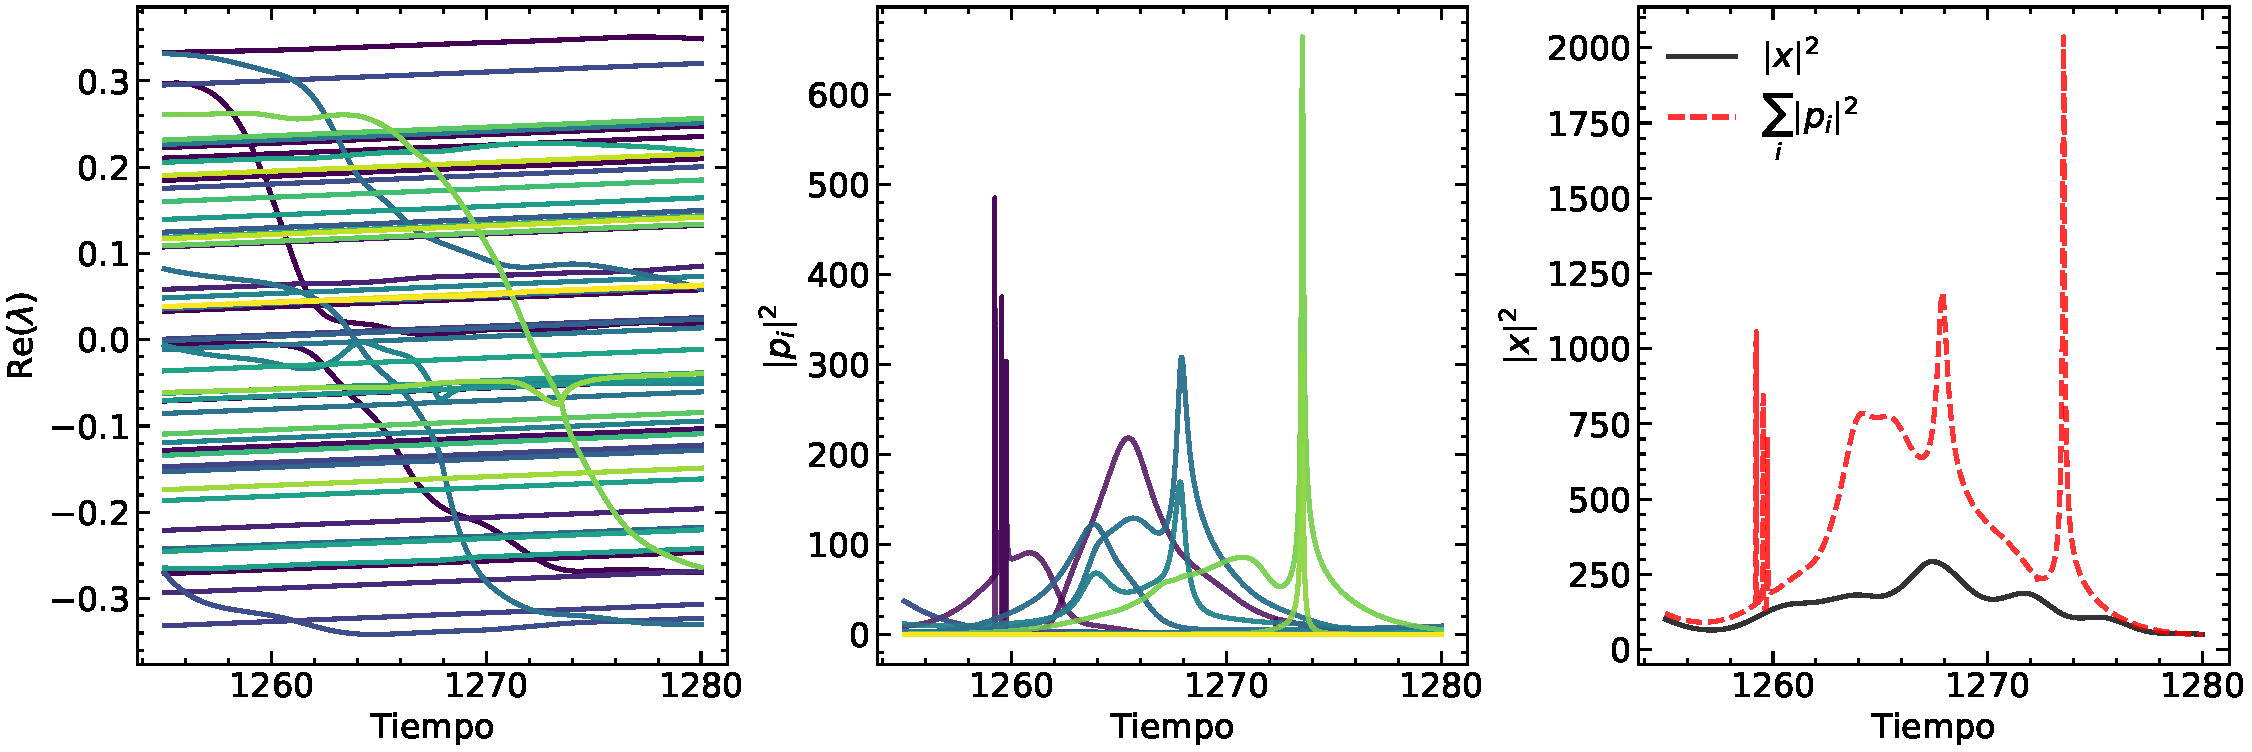
\includegraphics[width=\linewidth]{Figures/Picos_acoplados.pdf}
  \caption{\textbf{Izquierda:} Parte real de los autovalores en función del tiempo pasado el transitorio, se observa cómo la dinámica se aleja de las caídas limpias que se observan para dimensiones menores en la figura \ref{fig:picos}. \textbf{Centro:} Proyecciones de \(\mathbf{x}\) sobre los autovectores de \(W\) donde se observa que siguen estando, en su mayoría, descorrelacionados entre sí pero alejándose del comportamiento puramente oscilatorio para bajas dimensiones. \textbf{Derecha:} Norma al cuadrado de \(\mathbf{x}\) (negro) frente a la suma de los cuadrados de las proyecciones de \(\mathbf{x}\), donde se observa cómo ya difieren demasiado debido a que los términos cruzados se hacen no despreciables.}
  \label{fig:picos acoplados}
\end{figure}

La configuración que adquiere el sistema estructurando los autovalores de la matriz de conexiones en torno a \(\re(\lambda) = 0\), justo entre la región asintóticamente estable y la región inestable corresponde a lo que hemos denominado como criticidad dinámica, donde el estado crítico viene dado, no por un punto en el espacio de las fases, sino por un régimen dinámico.

\subsection{Modelo de aprendizaje antisimétrico simplificado}
Una vez obtenido un conocimiento profundo en cuanto a la dinámica de la red sin un término de aprendizaje retentivo, tan solo para estabilizarla en torno a un estado crítico en el sentido dinámico, se procede a estudiar cómo introducir un factor de aprendizaje antisimétrico afecta a la dinámica tanto a nivel de estabilidad como en la generación de patrones resistentes a la erosión anti hebbiana. Para ello nos basamos en el modelo obtenido por \textcite{susman2019} en el que proponen que el resultado de un aprendizaje mediante STDP se puede aproximar como una perturbación antisimétrica en la matriz de conexiones, sección \ref{sec:Aprendizaje anti simétrico y STDP}, por lo que nuestro término de aprendizaje de la ecuación \eqref{eq:evolución conexiones} sería

\begin{equation}
  \Delta_L = \rho (\mathbf{rs}^T - \mathbf{sr}^T)
\end{equation}

Podemos suponer sin pérdida de generalidad que \(\mathbf{r}\) y \(\mathbf{s}\) son un par de vectores ortonormales entre sí, ya que si no lo fuesen podríamos escribir \(\mathbf{r}\) y \(\mathbf{s}\) en función de una base ortonormal del plano generado por estos dos vectores, \(\{\tilde{\mathbf{r}}, \tilde{\mathbf{s}}\}\), siendo \(\mathbf{r} = a\tilde{\mathbf{r}} + b\tilde{\mathbf{s}}\) y \(\mathbf{s} = c\tilde{\mathbf{r}} + d\tilde{\mathbf{s}}\), por lo que podemos escribir el término antisimétrico en función de \(\tilde{\mathbf{r}}\) y \(\tilde{\mathbf{s}}\) como

\begin{equation}
  \Delta_L = \rho (\mathbf{rs}^T - \mathbf{sr}^T) = \rho (ad - bc)(\tilde{\mathbf{r}}\tilde{\mathbf{s}}^T - \tilde{\mathbf{s}}\tilde{\mathbf{r}}^T) = \rho |\mathbf{r}||\mathbf{s}|\sin\theta_{\mathbf{rs}}(\tilde{\mathbf{r}}\tilde{\mathbf{s}}^T - \tilde{\mathbf{s}}\tilde{\mathbf{r}}^T)
  \label{eq:antisimetría y ortogonalidad}
\end{equation}

Por tanto siempre podemos suponer \(\mathbf{r}\) y \(\mathbf{s}\) ortonormales y escalar con el correspondiente factor, en el caso de que no lo sean, notando que cuando ambos son colineales \(\sin \theta_{\mathbf{rs}} = 0\), por lo que es necesario que la matriz \(\Delta_L\) sea al menos de rango 2\footnote{De hecho una matriz antisimétrica solo puede tener rango par.}, haciendo que la evolución de \(W\) venga dada por 

\begin{equation}
  \dot{W} = \alpha [\mathbb{1} - \mathbf{xx}^T + \rho(\mathbf{rs}^T - \mathbf{sr}^T)]
\end{equation}


Para comprobar el efecto de añadir el término antisimétrico en la matriz de conexiones seguiremos la parte imaginaria del espectro antes, durante y después de la presentación del estímulo durante una ventana de tiempo, y comprobaremos la proyección del plano \(\mathbf{rs}\) sobre los planos generados por los autovectores asociados a cada par de autovalores complejos conjugados.

\begin{figure}[htbp]
  \centering
  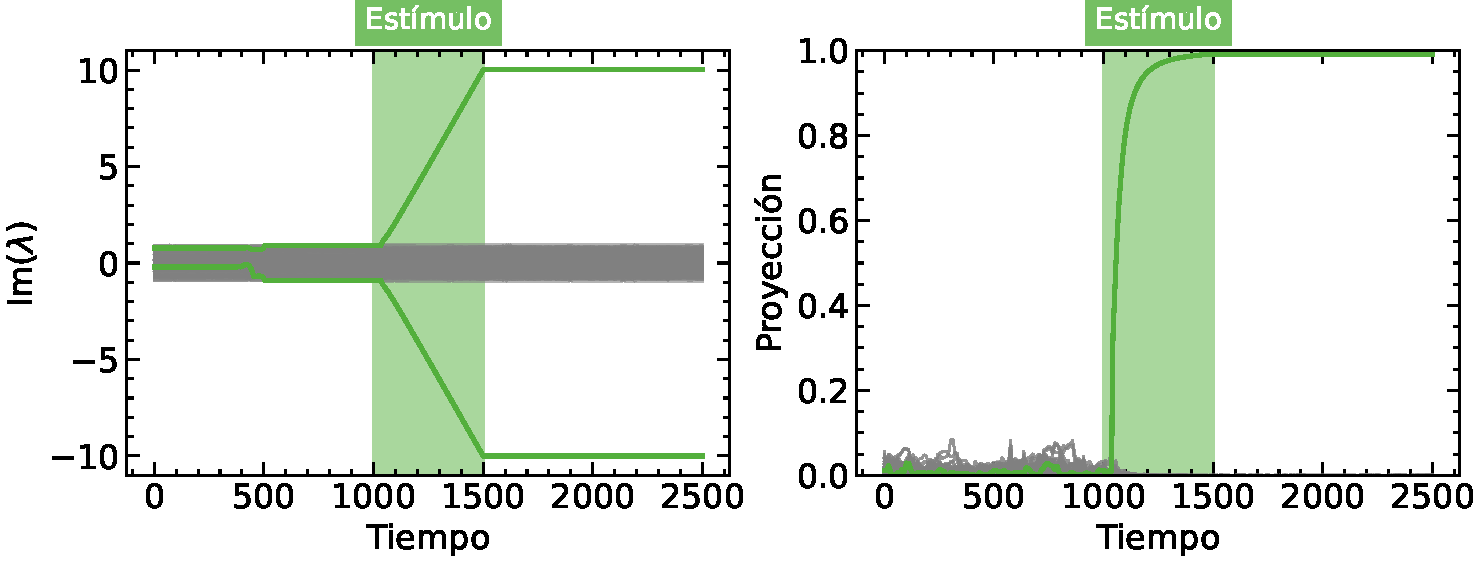
\includegraphics[width=\linewidth]{Figures/visualizacion estimulo.pdf}
  \caption{\textbf{Izquierda:} Parte imaginaria de los autovalores de la matriz de conexiones \(W\), antes, durante y después de la introducción del estímulo, se observa cómo antes y después la parte imaginaria del espectro es prácticamente constante en el tiempo, y cómo la retención de una memoria se expresa como el crecimiento en la amplitud imaginaria de un par de autovalores complejo conjugados. \textbf{Derecha:} Proyección del plano de los autovectores asociados al par de autovalores que retienen la memoria sobre el plano generdo por los vectores \(\mathbf{r}\) y \(\mathbf{s}\) frente a la proyección del mismo plano \(\mathbf{rs}\) sobre los \(\sim N/2-1\) planos generados por el resto de pares de autovectores asociados a pares de autovalores complejo conjugados. Se observa cómo la proyección del plano \(\mathbf{rs}\) sobre el de los autovectores de la memoria aumenta hasta casi 1, lo que muestra como los vectores \(\mathbf{r}\) y \(\mathbf{s}\) quedan codificados dentro de la matriz \(W\) de forma permanente tras el aprendizaje. Simulación para \(\alpha = 0.001\), \(N = 100\), \(\rho = 20\) y \(\Delta t_{Estimulo} = 500\).}
  \label{fig:aprendizaje antisimétrico}
\end{figure}

De forma similar al aprendizaje hebbiano, el aprendizaje antisimétrico es capaz de generar \emph{outliers} en los autovalores de la matriz de conexiones asociados a las memorias aprendidas, almacenando, además, información de los propios vectores memorizados en el proceso, figura \ref{fig:aprendizaje antisimétrico}. Además se puede observar cómo al aumentar el tiempo de presentación del estímulo la amplitud imaginaria de los autovalores de la memoria aumenta de forma lineal, mientras que la proyección de los autovectores de la memoria sobre los vectores memorizados se estanca en 1, por lo que un aumento en la amplitud de los autovalores, el tiempo de presentación del estímulo o la amplitud del estímulo no conlleva necesariamente una mayor retención de la memoria a partir del punto de estancamiento. 

Y al igual que en el modelo de Hopfield es posible introducir varias memorias diferentes dentro de una misma matriz de conexiones hasta un límite similar que en el modelo simétrico \parencite{susman2019}, como se puede observar en la figura \ref{fig:varias memorias}, donde se han introducido tres memorias con diferentes amplitudes \(\rho\) para observar cómo la eficacia de la red para almacenar patrones no depende solamente del número de neuronas, sino también del propio proceso de aprendizaje, que es capaz de corromper tanto las memorias ya almacenadas como la que estáen proceso de aprendizaje.

\begin{figure}[htbp]
  \begin{subfigure}[t]{0.48\linewidth}
    \caption{}
    \label{fig:memorias antisimetricas}
    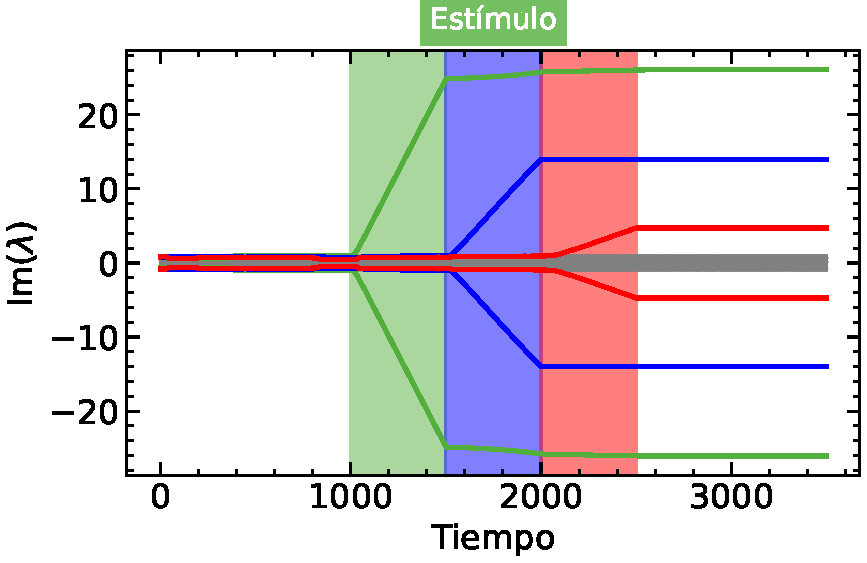
\includegraphics[width=\linewidth]{Figures/memorias antisimetricas.pdf}
  \end{subfigure}
  \hfill
  \begin{subfigure}[t]{0.48\linewidth}
    \caption{}
    \label{fig:proyecciones antisimetricas}
    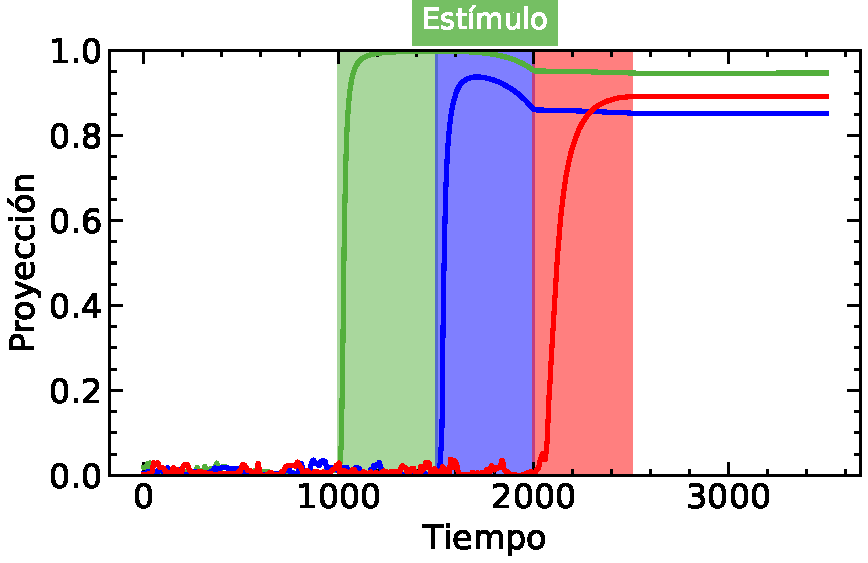
\includegraphics[width=\linewidth]{Figures/proyecciones antisimetricas.pdf}
  \end{subfigure}
  \hfill
  \begin{subfigure}[t]{0.48\linewidth}
    \caption{}
    \label{fig:memorias solapadas}
    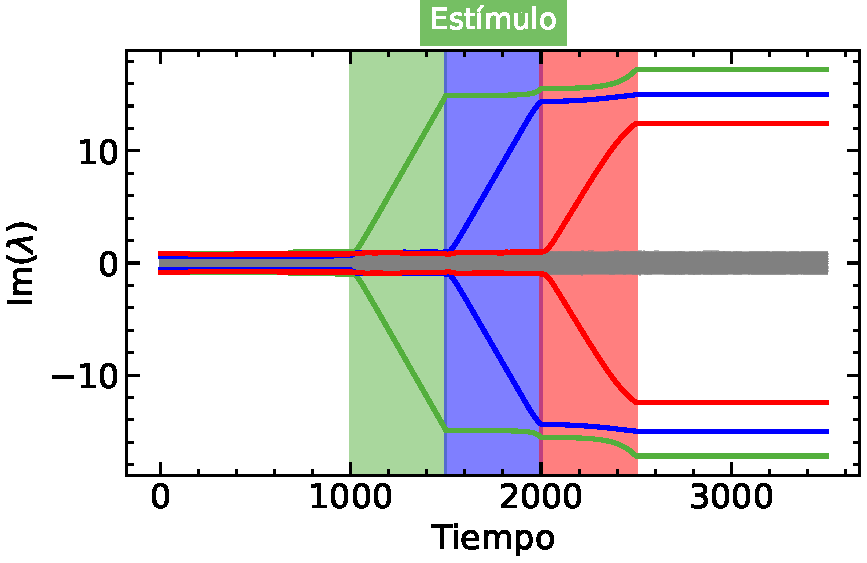
\includegraphics[width=\linewidth]{Figures/memorias solapadas.pdf}
  \end{subfigure}
  \hfill
  \begin{subfigure}[t]{0.48\linewidth}
    \caption{}
    \label{fig:proyecciones solapadas}
    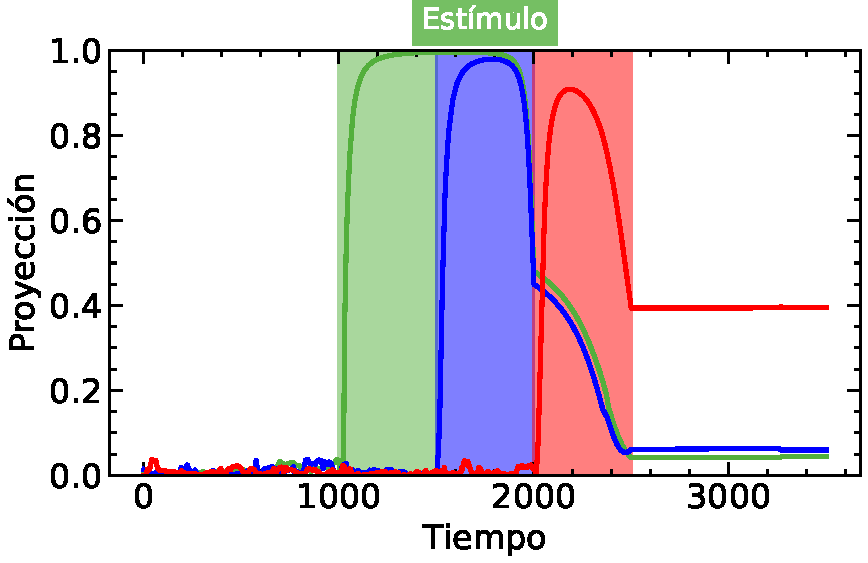
\includegraphics[width=\linewidth]{Figures/proyecciones solapadas.pdf}
  \end{subfigure}
  \caption{La capacidad de retención no depende solamente del número de memorias. La primera columna muestra la amplitud de la parte imaginaria de los autovalores de \(W\) antes, durante y después de la presentación de tres estímulos diferentes dados por los vectores \(\mathbf{r}^{(i)}\) y \(\mathbf{s}^{(i)}\) con \(i=1, 2, 3\), en \subref{fig:memorias antisimetricas} la amplitud del estímulo, \(\rho\) es diferente para cada uno de ellos y el tiempo de presentación el mismo, por lo que la amplitud alcanzada por cada autovalor es diferente, evitando que choquen entre sí, mientras que en \subref{fig:memorias solapadas} la amplitud del estímulo es el mismo, por lo que los autovalores chocan interactuando entre ellos. La segunda columna muestra la proyección de cada plano de la memoria aprendida con el plano generado por los vectores \(\mathbf{r}^{(i)}\) y \(\mathbf{s}^{(i)}\) empleados en el estímulo, en \subref{fig:proyecciones antisimetricas} al estar los autovalores separados entre sí las proyecciones se mantienen robustas a lo largo del tiempo, mientras que en \subref{fig:proyecciones solapadas} las interacciones entre autovalores modifican los autovectores de la memoria dañando esta y disminuyendo la proyección entre planos.}
  \label{fig:varias memorias}
\end{figure}

Una vez almacenada la memoria en la matriz de conexiones el siguiente paso lógico es buscar cómo extraer esa información y hacer que el conjunto de neuronas se estructure en un patrón similar al de la memoria aprendida, sin embargo aquí es donde nos encontramos con problemas, el primero es que a diferencia del modelo de Hopfield, no hay una configuración especial de \(\mathbf{x}\) que minimice la energía de la red pues si la tomamos como \eqref{eq:energia hopfield}

\begin{equation}
  E = -\frac{1}{2}\sum_{i,j}W_{ij}x_ix_j
\end{equation}

pero como para una matriz antisimétrica los términos cruzados \(W_{ij} = -W_{ji}\) se cancelan entre sí  la energía total asociada a la parte antisimétrica es 0, por lo que la evolución mediante la ecuación \eqref{eq:evolución actividad} no empuja a \(\mathbf{x}\) hacia ninguna dirección en concreto sino que hace que cada una de las proyecciones de \(\mathbf{x}\) sobre los autoplanos de \(W\)\footnote{Los \emph{autoplanos} son los planos generados por un par de autovectores complejo conjugados.} rote, por lo que a la hora de recuperar la memoria al introducir un estímulo en \(\mathbf{x}\) similar al patrón empleado no observaremos cómo todo el sistema se estructura para formar el patrón \(\mathbf{r}\) o \(\mathbf{s}\), sino que durante un corto periodo de tiempo veremos cómo el conjunto de neuronas oscilará en torno a ambos patrones con una frecuencia dada por la parte imaginaria del par de autovalores conjugados asociados a la memoria.

Debido a que las direcciones \(\mathbf{r}\) y \(\mathbf{s}\) han quedado codificadas de forma permanente en la matriz de conexiones en forma de autovectores, una vez que se excite al conjunto de neuronas mediante un estímulo lo suficientemente grande generado en el plano \(\mathbf{rs}\) de la forma \(\mathbf{h}(t) = p_\mathbf{r} \mathbf{r} + p_\mathbf{s} \mathbf{s}\), {\color{blue}insertándolo en la ecuación \ref{eq:evolución actividad} de la forma

\begin{equation}
  \dot{\mathbf{x}} = W\mathbf{x} + \mathbf{h}(t)
\end{equation}}
al ser \(\mathbf{r}\) y \(\mathbf{s}\) vectores propios de la matriz de conexiones con autovalores \(\lambda = -\beta \pm i \rho\) la actividad neuronal evolucionará, si \(\mathbf{h}(t) \ll \mathbf{x}_{\text{sin excitar}}\), como 

\begin{equation}
  \dot{\mathbf{x}} = W\mathbf{x} \simeq W\mathbf{h} = p_\mathbf{r} W\mathbf{r} + p_\mathbf{s} W\mathbf{s} \Rightarrow
  \begin{cases}
    p_\mathbf{r}(t) \simeq e^{-\beta + i\rho}p_\mathbf{r}(0)\\
    p_\mathbf{s}(t) \simeq e^{-\beta - i\rho}p_\mathbf{s}(0)
  \end{cases}
\end{equation}
donde \(p_{\mathbf{r/s}}\) son las proyecciones sobre las direcciones \(\mathbf{r}\) y \(\mathbf{s}\), por ello al medir la proyección de \(\mathbf{x}\) sobre la dirección \(\mathbf{r}\) aparecerá una reverberación del estímulo que se extenderá después de haberse apagado este, y que solo aparecerá en la proyección de la dirección del estímulo y no en el resto de direcciones. 

\begin{figure}[htbp]
  \centering
  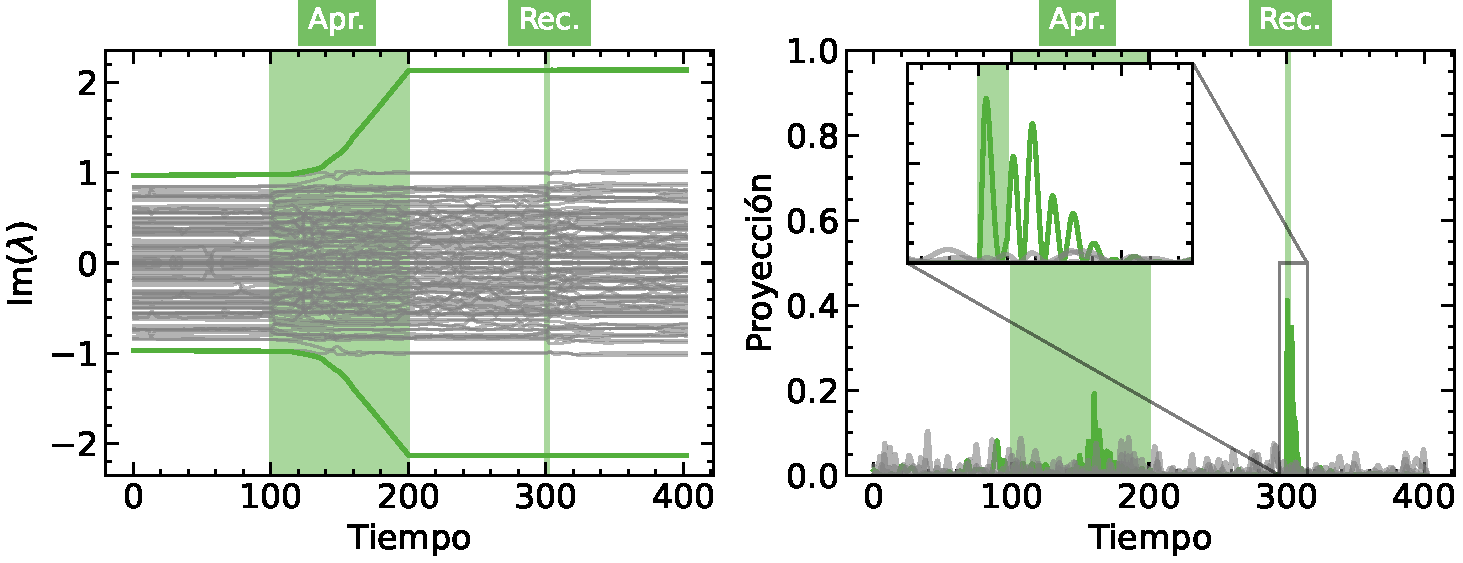
\includegraphics[width=\linewidth]{Figures/retrieval.pdf}
  \caption{Un estímulo en la dirección de la memoria introducida reverbera durante un tiempo. \textbf{Izquierda:} Amplitud imaginaria de los autovalores de \(W\) antes, durante y después del aprendizaje y de la recuperación, se observa cómo la recuperación de la memoria afecta mínimamente a su estado en la aprte imaginaria del autovalor. \textbf{Derecha:} En el momento en el que se aplica el estímulo externo la proyección de \(\mathbf{x}\) sobre \(\mathbf{r}\) aumenta, sin embargo esta no desaparece al eliminar el estímulo sino que revebera durante cierto tiempo antes de desaparecer, haciendo oscilar a \(\mathbf{x}\) entre \(\mathbf{r}\) y 
  \(\mathbf{s}\).}
  \label{fig:retrieval}
\end{figure}

\subsection{Modelo de aprendizaje con STDP}
El modelo de codificación de memorias presentado en la sección anterior se trata de una simplificación del modelo que buscamos simular, el STDP, ya que aunque a nivel matemático mediante ambos procesos estamos alimentando a la dinámica de la matriz de conexiones con una matriz antisimétrica, en el modelo simplificado introducimos directamente la matriz con el patrón ya estructurado en la dinámica, algo que a nivel neurológico no es plausible, ya que si buscamos hacer una analogía con el comportamiento real de las neuronas en el cerebro, la dinámica de las conexiones no puede ser modificada conexión a conexión sino que esta es una propiedad emergente de la dinámica de un gran número de neuronas. Para ello recuperamos la idea presentada en la sección \ref{sec:Aprendizaje anti simétrico y STDP}, donde la verdadera dinámica de aprendizaje de \(W\) es 

\begin{align}
  \Delta_L &= \eta (\mathbf{xy}^T - \mathbf{yx}^T)\\
  \dot{\mathbf{y}} &= \frac{1}{\tau} (\mathbf{x-y})
\end{align}

donde \(\mathbf{y}(t)\) puede ser expresado en función de \(\mathbf{x}(t)\) como un integrador con fugas de tiempo característico \(\tau\)

\begin{equation}
\mathbf{y}(t) =\frac{1}{\tau}\int_{t_0}^t\underbrace{e^{(t'-t)/\tau}}_{\substack{\text{Kernel}\\\text{exponencial}}}\mathbf{x}(t')dt' + \underbrace{\mathbf{y}(t_0)e^{(t_0-t)/\tau}}_{\substack{\text{Fase inicial que}\\\text{disminuye exponencialmente}}}
\end{equation} 

Cuando presentamos la dinámica STDP comentamos que cuando el estímulo que se le presenta a la red se mueve en el plano generado por los vectores \(\mathbf{r}\) y \(\mathbf{s}\) podemos aproximar el término de aprendizaje que depende del tiempo por un término constante en forma de una matriz antisimétrica generada mediante \(\mathbf{r}\) y \(\mathbf{s}\). Sin embargo para que ello sea posible el estímulo no puede ser de cualquier tipo ya que los vectores \(\mathbf{x}\) e \(\mathbf{y}\) deben ser ortogonales o al menos linealmente independientes para poder encontrar una matriz no nula dada por la ecuación \eqref{eq:antisimetría y ortogonalidad}, esto es \(\sin\theta_{\mathbf{xy}} \neq 0\), y aquí es donde entra en juego el método de cálculo de \(\mathbf{y}\), pues se trata de un integrador con fugas de \(\mathbf{x}\) que actúa promediando el vector de actividad neuronal en una ventana de tiempo mediante una función exponencial dándole más peso a los tiempos cercanos y menos a los lejanos con un tiempo característico \(\tau\), por lo que a tiempo \(t\) todo lo que haya ocurrido a tiempos mucho más antiguos que \(\sim t - \tau\) no tendrá relevancia \footnote{-2.3\(\tau\) supone el percentil 90 de la distribución, por lo que ocurra a tiempos anteriores será solo un 10\% del valor total, siendo la escala de tiempos que \emph{recuerda} \(\mathbf{y}\) del orden de \(\tau\).}, y todo lo que ocurra dentro de ese rango de tiempos entre \(t-\tau\) y \(t\) se promediará entre sí.

\begin{figure}[htbp]
  \centering
  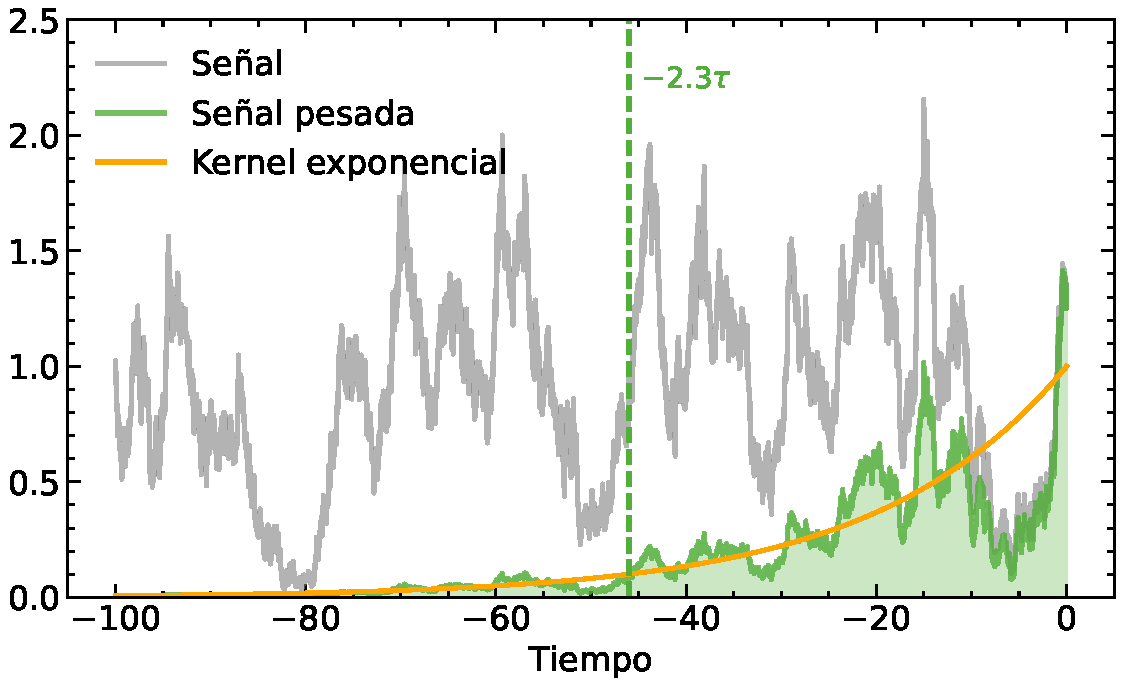
\includegraphics[width=0.8\linewidth]{Figures/leaky integrator.pdf}
  \caption{{\color{blue}Efecto del integrador con fugas. La trayectoria gris es la señal original, \(\mathbf{x}\), mientras que la verde es la señal pesada por el \emph{kernel} exponencial, \(e^{-t/\tau}\mathbf{x}\). Los valores a tiempos menores a \(\sim 2.3 \tau\) no afectan al cómputo total del integrador, \(\mathbf{y}\), el área sombreada en verde.}}
\end{figure}

Una vez mostrado esto, queda claro que si el tiempo en que se presenta el estímulo es mucho menor al tiempo característico, \(\tau\), este se \emph{perderá} en el promedio, por lo que solo serán significativos estímulos externos que duren tiempos mayores a \(\tau\). Sin embargo un estímulo uniforme no producirá una matriz antisimétrica, pues si aplicamos el estímulo \(\mathbf{h}(t) = \mathbf{h}\) durante el tiempo suficiente ocurrirá que tanto \(\mathbf{x} = \mathbf{h}\) como \(\mathbf{y} = \mathbf{h}\), por lo que \(\mathbf{xy}^T - \mathbf{yx}^T = \mathbf{hh}^T - \mathbf{hh}^T = 0\), esto tiene sentido ya que lo que estamos intentando introducir en la memoria de la red no es un solo patrón sino un conjunto de dos patrones ortogonales, por lo que el estímulo requerirá de cierta \emph{dinámica} en el plano de los patrones para poder separar \(\mathbf{x}\) e \(\mathbf{y}\) lo suficiente como para producir una matriz antisimétrica. Aquí es donde \textcite{susman2019} proponen un estímulo genérico de la forma \(\mathbf{h}(t) = \eta(t) \mathbf{r} + \xi(t) \mathbf{s}\), con \(\eta(t)\) y \(\xi(t)\) sendos ruidos blancos de amplitud \(\sigma\) para generar un camino aleatorio por el plano \(\mathbf{rs}\) que capture la geometría del espacio. Con este modelo aseguran obtener resultados similares a los obtenidos en la sección anterior (separación  de un par de autovalores \emph{outliers} complejo conjugados con autovectores pertenecientes al plano \(\mathbf{rs}\)), sin embargo mediante una revisión de su código y de los parámetros empleados en su simulación uno es capaz de constatar que dicho resultado no es replicable dado que depende fuertemente de la semilla elegida para generar el ruido aleatorio, figura \ref{fig:susman}. Con esto no se pretende plantear la invalidez de dicho resultado sino puntualizar el hecho de que no es tan general como se da a entender y que el estímulo necesario para producir los resultados esperados no es tan genérico como se plantea inicialmente.

\begin{figure}[htbp]
  \begin{subfigure}[t]{0.48\textwidth}
    \caption{}\label{fig:seed seed}
    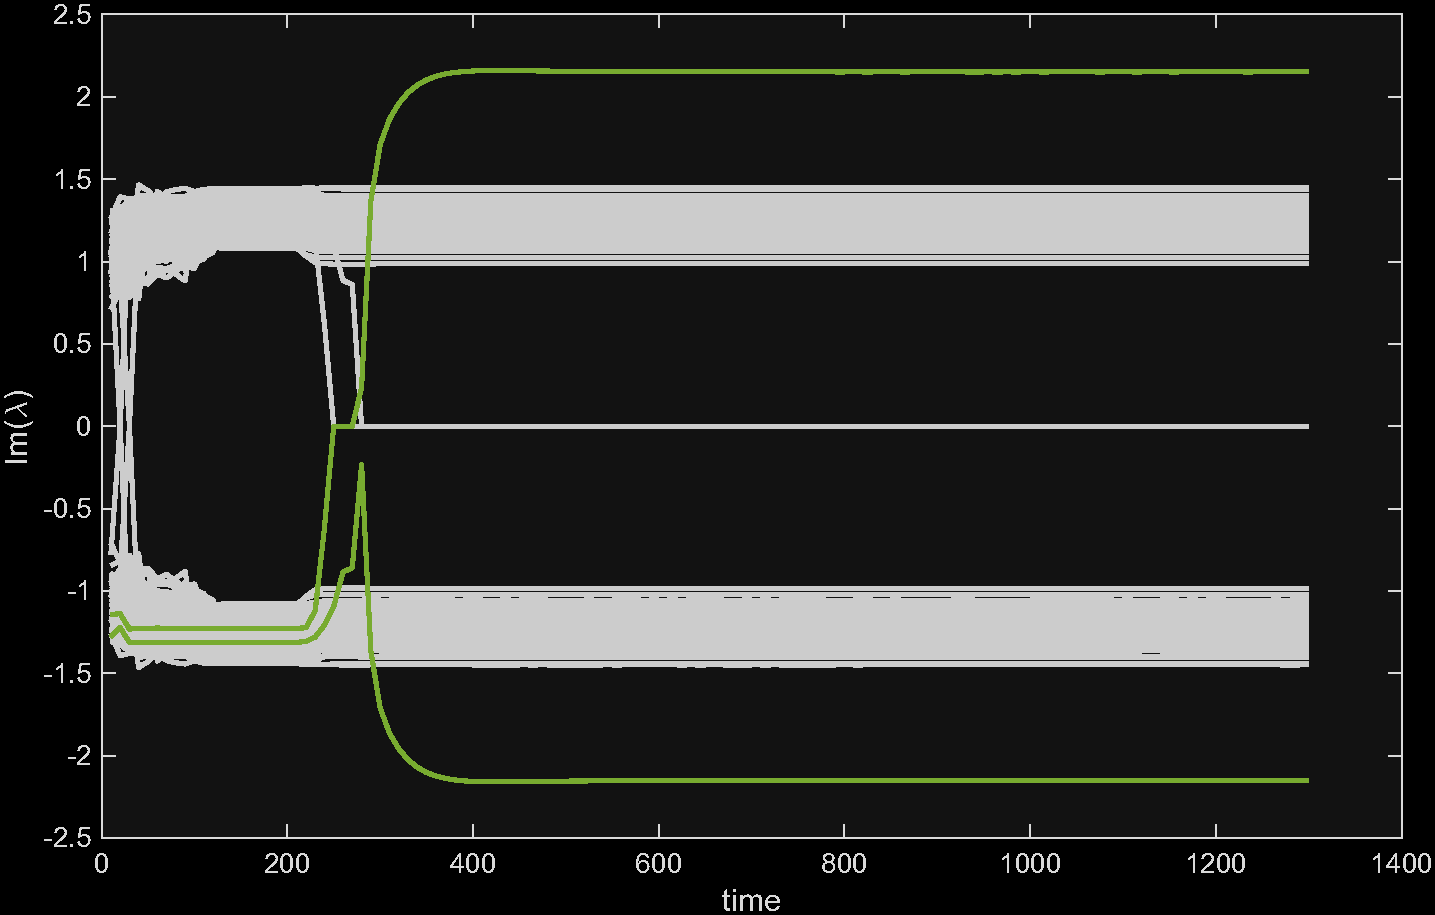
\includegraphics[width=.8\linewidth]{Figures/Figuras Susman/seed seed.pdf}
  \end{subfigure}
  \hfill
    \begin{subfigure}[t]{0.48\textwidth}
    \caption{}\label{fig:seed 6342643}
    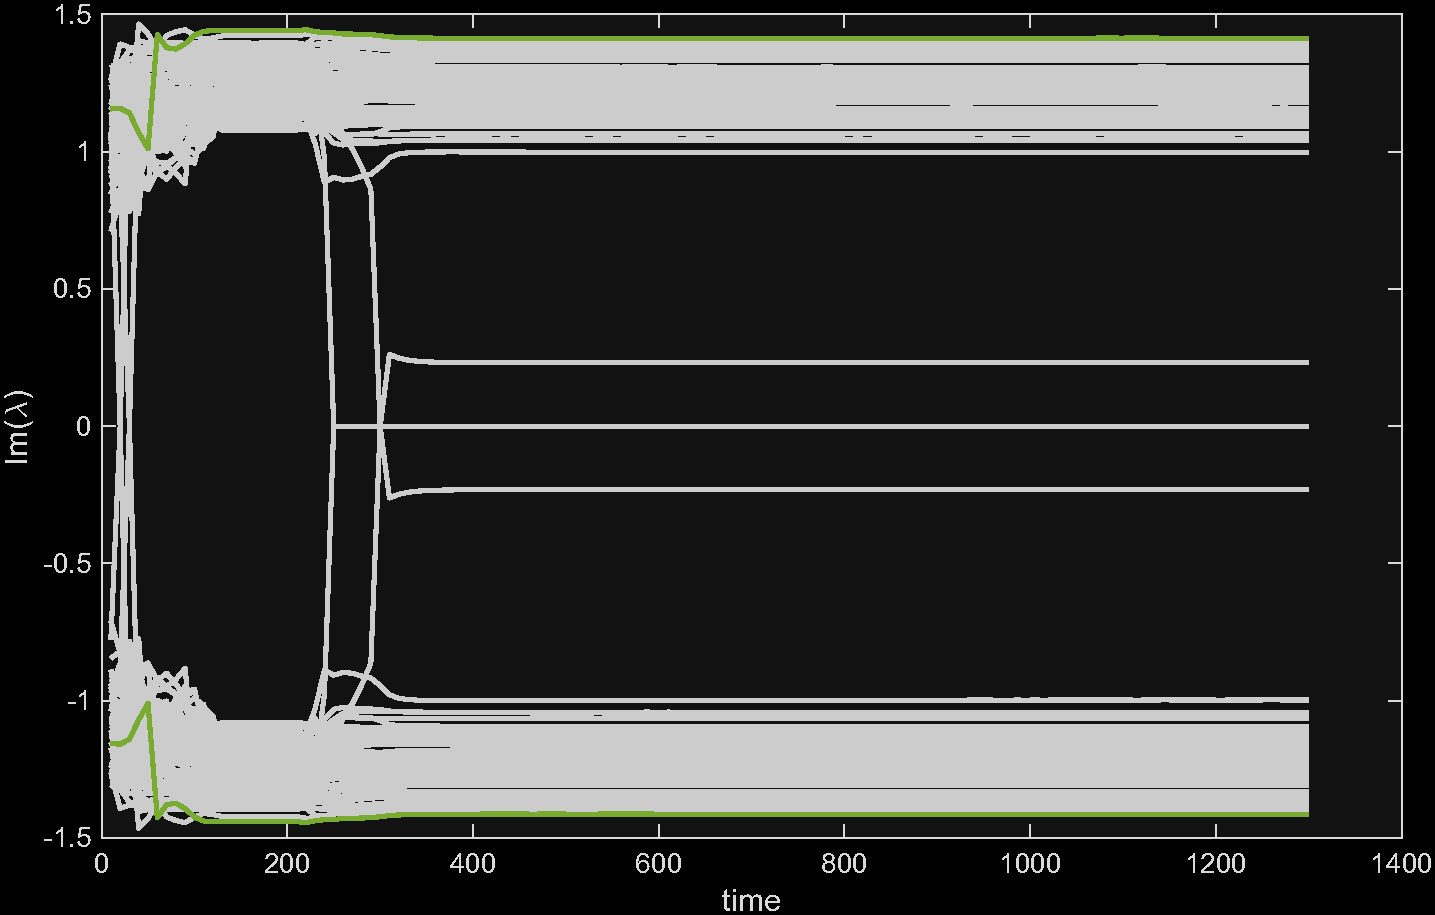
\includegraphics[width=.8\linewidth]{Figures/Figuras Susman/seed 6342643.pdf}
  \end{subfigure}
  \hfill
    \begin{subfigure}[t]{0.48\textwidth}
    \caption{}\label{fig:seed 56734}
    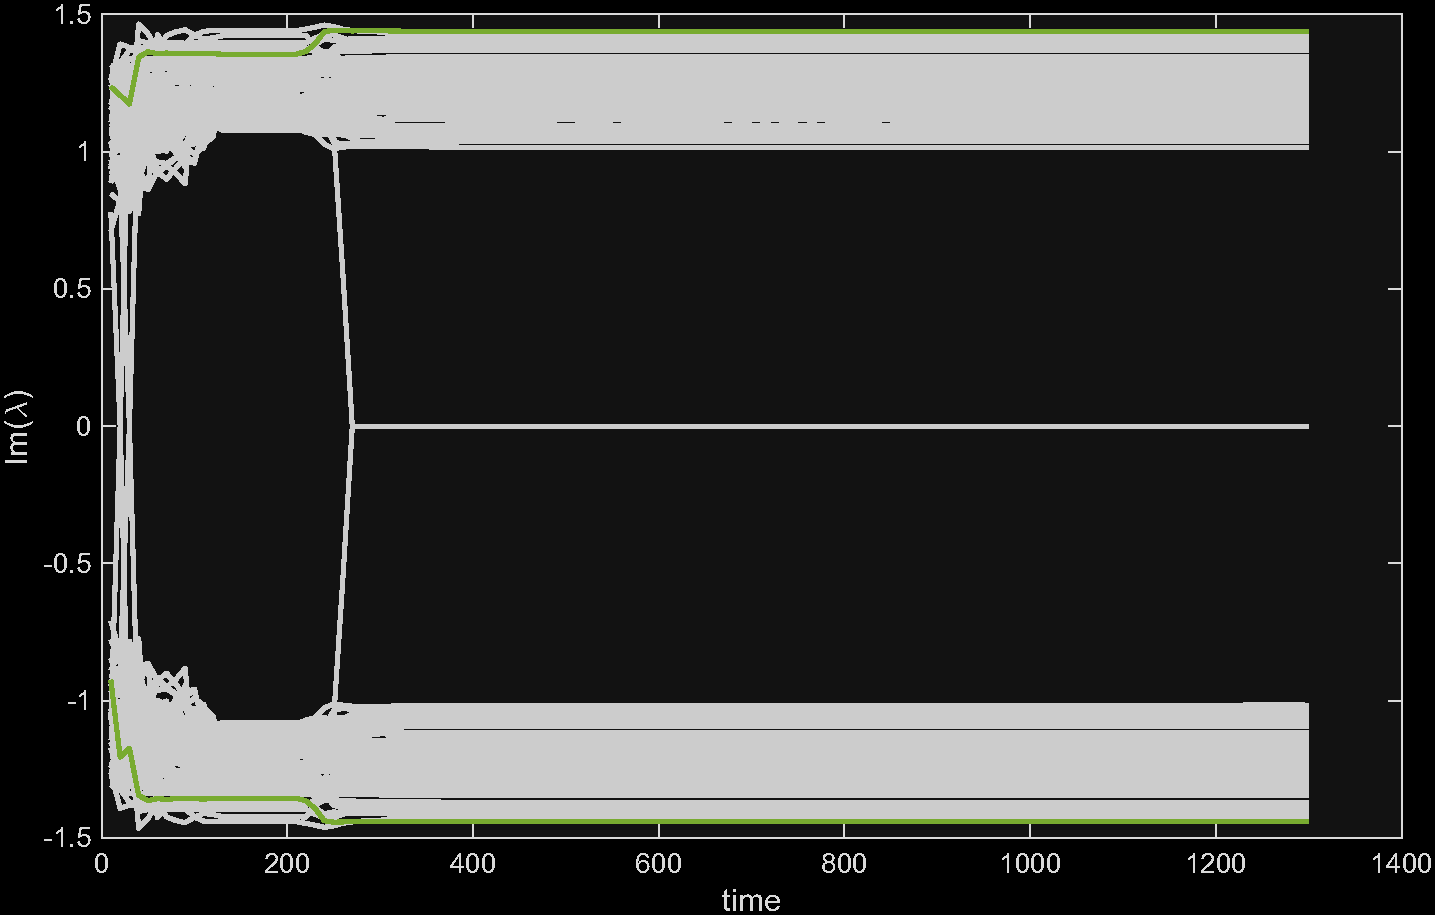
\includegraphics[width=.8\linewidth]{Figures/Figuras Susman/seed 56734.pdf}
  \end{subfigure}
  \hfill
    \begin{subfigure}[t]{0.48\textwidth}
    \caption{}\label{fig:seed 11}
    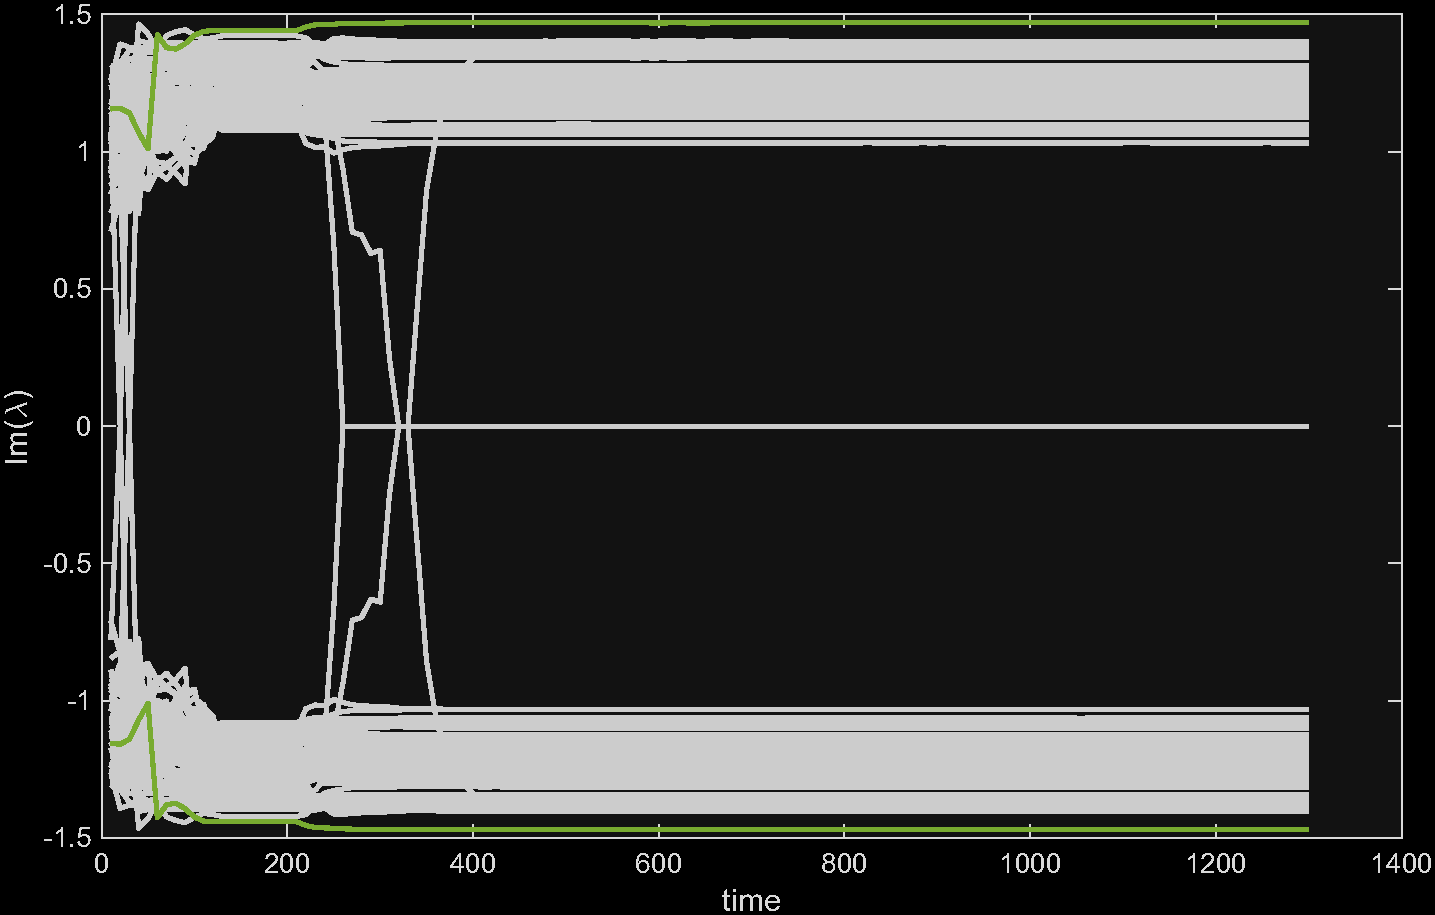
\includegraphics[width=.8\linewidth]{Figures/Figuras Susman/seed 11.pdf}
  \end{subfigure}
  \caption{El caminante aleatorio no proporciona un estímulo valioso. En esta figura se muestran cuatro realizaciones del proceso de aprendizaje mediante STDP, la subfigura superior izquierda, \subref{fig:seed seed}, presenta el comportamiento esperado del modelo antisimétrico, mostrando la separación en la parte imaginaria de un par de autovalores complejo conjugados, mientra que las otras tres subfiguras, \subref{fig:seed 6342643}, \subref{fig:seed 56734} y \subref{fig:seed 11}, cuyas semillas del generador de números aleatorios han sido seleccionadas de forma aleatoria no muestran el comportamiento esperado. Los resultados se han obtenido empleando el código proporcionado por \parencite{susman2019} en el propio artículo eliminando los términos no lineales de \(\tanh(\mathbf{x})\).}
  \label{fig:susman}
\end{figure}


{\color{blue}
  Es necesario matizar que el estudio que se lleva a cabo en \textcite{susman2019} del sistema con aprendizaje STDP y homeostásis anti hebbiana difiere del realizado en este trabajo en que ellos toman una función activadora \(\phi(\mathbf{x})\) y dinámica estocástica.

\begin{align}
  \dot{\mathbf{x}} &= W\phi(\mathbf{x}) + \mathbf{h}(t) + \bm{\xi}(t)\\
  \dot{W} &= \alpha (\mathbb{1} - \phi(\mathbf{x})\phi(\mathbf{x})^T  + \phi(\mathbf{x})y - \mathbf{y}\phi(\mathbf{x})^T) + \eta(t) \\
  \dot{\mathbf{y}} &= \frac{1}{\tau}(\phi(\mathbf{x}) - \mathbf{y})
\end{align}

El caso lineal, \(\phi(\mathbf{x})=\mathbf{x}\), y determinista, \(\bm{\xi}(t) = 0\) y \(\eta(t) = 0\), en vez de ruido estocástico, es el que se contempla en este trabajo obteniendo los resultados mostrados, sin embargo en \parencite{susman2019} se toma \(\phi(\mathbf{x}) = \tanh(\mathbf{x})\), representando la tasa de disparo de cada neurona en vez de su actividad, generando una saturación en \(|\mathbf{x}| = \sqrt{N}\), a pesar de esto la dinámica presentada genera los mismos resultados independientemente de la función de activación (de entre las dos mostradas) y se ha comprobado que la imposibilidad de generación de pares de autovalores de forma sistemática mediante un estímulo ruidoso también se cumple en este caso.
}

El hecho de que el ruido aleatorio descorrelacionado temporalmente no sea capaz de generar un patrón memorizable es tan sencillo como que el promedio temporal del ruido blanco es 0, y por tanto al ser \(\mathbf{y}\) un promedio de \(\mathbf{x}\), y por tanto del estímulo \(\mathbf{s}(t)\) durante el tiempo en el que se presenta, este vector se hará 0 y por tanto no habrá perturbación antisimétrica.

Para que la matriz realmente capture la estructura del plano \(\mathbf{rs}\) se debe cumplir tanto que \(\mathbf{y}\) sea diferente de 0 como que sea diferente de \(\mathbf{x}\), y esto es posible tan solo si el vector \(\mathbf{h}(t)\) rota en el plano \(\mathbf{rs}\) en un sentido específico, esto es \(\mathbf{h}(t) \simeq \sin(\omega t)\mathbf{r} + \cos(\omega t)\mathbf{s}\). Si \(\mathbf{h}(t)\) representa una rotación en el plano \(\mathbf{rs}\), al ser \(\mathbf{y}\) una imagen desfasada de \(\mathbf{x}\), este primero será linealmente independiente al segundo durante todo el proceso de estimulación, generando una matriz no nula, aún así si la frecuencia angular de rotación de \(\mathbf{s}(t)\) en el plano \(\mathbf{rs}\), \(\omega\) es mucho mayor a \(\frac{2\pi}{\tau}\), \(\mathbf{x}\) realizará más de una rotación completa durante el tiempo en el que \(\mathbf{y}\) está promediando, por lo que por pura geometría al ser el promedio de un vector a lo largo  de una rotación completa 0, \(\mathbf{y}\) volverá a ser nulo, o despreciable de forma similar a cuando había ruido aleatorio, por eso no solo \(\mathbf{s}(t)\) debe rotar en el plano \(\mathbf{rs}\), sino que debe hacerlo con una frecuencia angular \(\omega \simeq \frac{2\pi}{\tau}\), mucho mayor y \(\mathbf{y}\) se hace 0, mucho menor y el estímulo es prácticamente constante en el tiempo, haciendo \(\mathbf{y} \simeq \mathbf{x}\), y por tanto \(\mathbf{xy}^T-\mathbf{yx}^T \simeq 0\).

\begin{figure}[htbp]
  \centering
  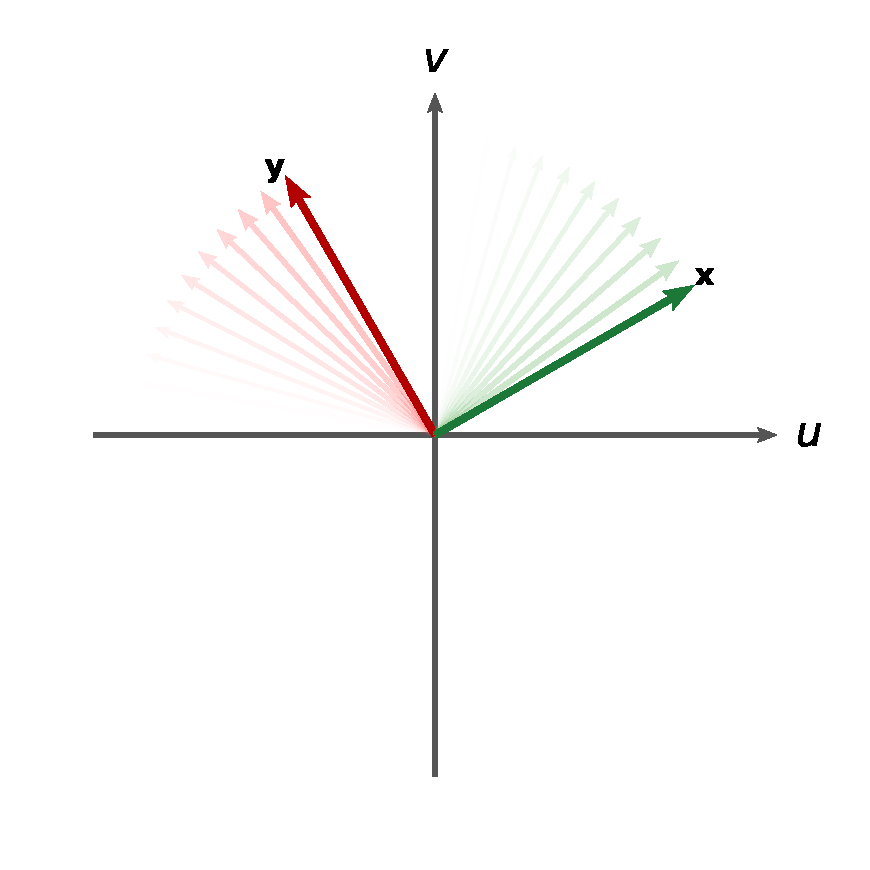
\includegraphics[width=0.6\linewidth]{Figures/rotacion.pdf}
  \caption{\(\mathbf{x}\) e \(\mathbf{y}\) deben estar desfasados en su rotación en el plano \(\mathbf{rs}\) para poder generar una matriz antisimétrica mediante el aprendizaje basado en el STDP.}
\end{figure}

\begin{figure}[htbp]
  \centering
  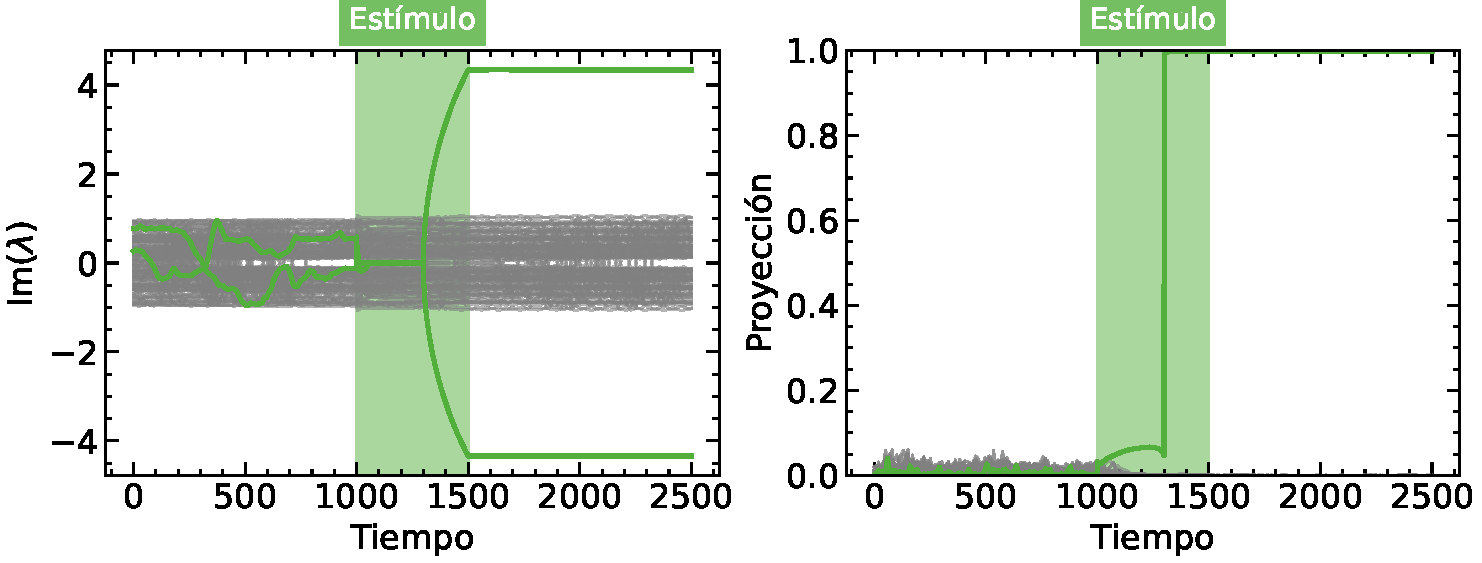
\includegraphics[width=\linewidth]{Figures/STDP correcto.pdf}
  \caption{El aprendizaje STDP es capaz de generar \emph{outliers} imaginarios. \textbf{Izquierda:} Parte imaginaria de los autovalores de la matriz de conexiones. Se observa claramente como el parendizaje basado en la STDP genera un aumento en la amplitud imaginaria de un par de autovalores complejo conjugados de forma similar a cómo ocurre con la regla simplificada observada en la figura \ref{fig:aprendizaje antisimétrico} pero con un crecimiento no lineal en la amplitud imaginaria. \textbf{Derecha:} Proyección del plano de los autovectores asociados a los autovalores \emph{outliers} sobre el plano \(\mathbf{rs}\). Al igual que en la figura \ref{fig:aprendizaje antisimétrico} aparece un punto en el que la proyección satura en 1 y por mucho que aumente la parte imaginaria del autovalor no aumenta la proyección entre planos. Simulación para \(\alpha = 0.001\), \(N=10\), \(\rho=50\), \(\Delta t_{Estimulo}=500\), \(\tau=500\) y \(\omega = \frac{\pi}{\tau}\).}
  \label{fig:aprendizaje STDP}
\end{figure}
La figura \ref{fig:aprendizaje STDP} muestra claramente cómo mediante un estímulo \emph{giratorio} el aprendizaje de la memoria se lleva a cabo y de forma más intensa si tenemos en cuenta el salto en la proyección entre el plano de la memoria y el plano \(\mathbf{rs}\), pues en el caso del aprendizaje mediante una matriz antisimétrica preconstruida, figura \ref{fig:aprendizaje antisimétrico}, el crecimiento en la proyección es rápido y luego se suaviza hasta casi estancarse en 1, mientras que en el STDP el salto desde \(\sim 0\) hasta 1 es abrupto, mostrando que el método que almacena la memoria lo hace de forma más eficiente y no requiere que los autovalores de la memoria tengan un a parte imaginaria tan grande como en el caso del aprendizaje simplificado.

\section{Conclusions}
This Final Year Project has served to study and unpick the anti-Hebbian neural dynamics model in depth, not only by expanding on existing research into how this rule structures neural activity within a regime of dynamic criticality \parencite{magnasco2009} and how it is possible to harness the structure of homeostasis to store robust memories within changing connections \parencite{susman2019}, but also by delving into the specific conditions under which all this is possible and obtaining qualitative and quantitative results that explain the details of the various events arising from the dynamics at different scales.

The observable fact of the constant change in the synapses between neurons and in the connections they share has inspired the study of how dynamics might exist that are capable of keeping neuronal activity under control, whilst at the same time leaving room for mechanisms capable of transforming external stimuli into robust patterns encoded within the changing and mutable connections themselves. The homeostatic dynamics proposed in this final-year project utilise the symmetric part of the connection matrix which, as has been shown, dominates the real part of the eigenvalues of the system’s Jacobian, thereby enabling the system’s stability to be modified in order to obtain dynamics which, despite never reaching equilibrium, as observed in biological neural networks, maintains its activity within bounded limits, capable of responding to stimuli that might destabilise the network by adjusting the eigenvalues necessary to prevent this. This is the result of the \emph{struggle} between the network’s modes to gain control of the activities, and how an increase in the activity of one mode causes a consequent decrease in another, causing them to oscillate as they interact with one another.

{\color{blue}
This mechanism has enabled the system to organise itself into a semi-stable state, whilst, drawing inspiration from established methodology in the field—such as the Hopfield model— a method has been introduced to systematically embed patterns permanently within the structure of the connections themselves, without the need to modify them one by one. This has resulted in a relatively simple system of equations from which complex dynamics can emerge, rich in phenomena typical of self-organisation in complex systems, such as dynamics at the edge of criticality.

And, drawing inspiration from the Hopfield model, this work successfully reproduces different methods of permanently encoding memories within the network, both by embedding them directly in a manner more akin to Hopfield’s approach using an antisymmetric matrix, and by utilising the dynamics of the stimulus alongside those of the connections via Firing-Time-Dependent Plasticity to introduce the memories in the form of a pair of complex-conjugate eigenvalues and their respective eigenvectors, thereby refining and clarifying the model proposed by other researchers and elucidating its operation.

During the process of creating this work, we have explored well-established aspects of the study of neural networks and neural dynamics, such as the various methods of neural network learning that utilise connection dynamics, or anti-Hebbian homeostasis, relating them to cutting-edge topics that are at the forefront of current research, such as dynamic criticality and self-organisation, which leaves a great many questions open and avenues for further research. Some natural extensions of this work involve attempting to implement real synaptic dynamics, such as the existence of inhibitory and excitatory neurons—whose function determines the type of connection they form with others—and investigating the results obtained from a study using mean-field theory of the network at the limit of a large number of neurons, which is computationally very costly, such as the Wilson–Cowan model; and modifying the connection matrix to make it richer in structures, such as \emph{small world} or \emph{scale-free} networks, in a manner similar to how these appear at different scales in the brain, in order to analyse whether this alters critical or learning properties in any way.

\printbibliography

\end{document}